\documentclass[11pt,a4paper]{article}
\usepackage[margin=1in]{geometry}
\usepackage{amsmath,amssymb,amsthm,bm}
\usepackage{graphicx,booktabs,multirow}
\usepackage[table]{xcolor}
\usepackage{siunitx}
\usepackage[colorlinks=true,linkcolor=blue!60!black,citecolor=blue!60!black,urlcolor=blue!60!black]{hyperref}
\usepackage{enumitem}
\setlist{nosep}

\newtheorem{theorem}{Theorem}
\newtheorem{lemma}{Lemma}
\newtheorem{proposition}{Proposition}
\theoremstyle{remark}
\newtheorem{remark}{Remark}

\newcommand{\Tr}{\mathrm{Tr}}
\newcommand{\Var}{\mathrm{Var}}
\newcommand{\Cov}{\mathrm{Cov}}
\newcommand{\Bin}{\mathrm{Bin}}
\newcommand{\PS}{\mathrm{PS}}
\newcommand{\all}{\mathrm{all}}
\newcommand{\acc}{\mathcal{A}}
\newcommand{\id}{\mathbb{1}}
\newcommand{\calL}{\mathcal{L}}
\newcommand{\calP}{\mathcal{P}}
\newcommand{\vis}{\mathrm{vis}}
\newcommand{\inv}{\mathrm{inv}}

\title{Detection-driven extrapolation with twirled Pauli checks:\\ theory and a numerical comparison on deep Trotter circuits}
\author{Working notes --- October 2026}
\date{}

\begin{document}
\maketitle

\begin{abstract}
Post-selection on Pauli checks removes only the faults that anticommute with the checks, so by itself it is a projection of the noise rather than a uniform rescaling, and the post-selected observable depends on which faults the particular checks happen to see. We show that randomizing the check flavor uniformly over the non-identity Paulis on its support turns detection into a fair coin: every fault visible to the check is flagged with the same probability, whatever its Pauli type. Under this ``detection twirl'' the accepted state is an exact convex mixture of the fault-free state and the unmitigated state, with a mixing weight that is measured rather than modeled. Every acceptance rule then lies on one straight line, two points determine the fault-free value, and the extrapolation is exact to all orders for arbitrary stochastic Pauli noise. When faults are visible to different subsets of the checks, the accepted data decompose into species with known survival factors, and the fault-free value is recovered by a linear inversion over several acceptance rules. We relate these statements to the Pauli-path reactivity framework and verify them numerically on Clifford circuits. We then compare, on a transverse-field Ising Trotter circuit of 20 to 160 two-qubit gates with $1\%$ gate and readout error, standard zero-noise extrapolation, fixed Pauli checks with full post-selection, and the twirled-check protocol. The twirled protocol has the smallest bias at every depth, reaches a root-mean-square error of $0.02$ with $10^{3}$ to $10^{6}$ shots where exponential zero-noise extrapolation cannot reach it beyond depth 10 and fixed checks never do, and requires one noise rate per gate (the rotation-axis fault that no compatible check can see) instead of a full noise model; allowing every check flavor and repairing the rotations with controlled-$X$ gates removes even that rate at the price of extra gadget noise. Scanning the gate and readout error from $1\%$ to $0.2\%$ shows that the check-based protocols are unbiased at every noise level and that their cost relative to zero-noise extrapolation is a function of the clean fraction $q_0$ alone, with break-even at $q_0\approx0.3$: detection-driven extrapolation is cheaper than exponential zero-noise extrapolation when the checked circuit carries about one expected fault or fewer, $(g_p+g)\,p\,d\lesssim1.3$ for $g_p$ payload and $g$ gadget two-qubit gates per layer, i.e.\ $pd\lesssim0.06$ for the repaired gadget, and it is unbiased above that threshold at a cost that grows as $q_0^{-2}$. No threshold in the gate error alone exists for any of these methods, since every cost exponent is proportional to $pd$; what is depth- and error-independent is the comparison of exponents, which favours checks over ZNE with maximum gain $G_{\max}$ only if the gadget overhead ratio $r$ and the observable sensitivity $\kappa$ satisfy $1+r<G_{\max}\kappa$, a condition that two-sided checks on a local observable fail and observable-targeted, gate-efficient checks can meet. In error-detecting codes, where the detectors exist anyway, the same logic gives an exact geometric law $E[o\mid k]=O_0\bar\rho^{\,k}$ for the logical observable conditioned on the number $k$ of detected faults, which turns full post-selection into a regression over all shots with effective shot count $N\alpha_0^{1-\bar\rho^2}$ instead of $N\alpha_0$.
\end{abstract}

\tableofcontents

\section{Setting and notation}
\label{sec:setting}

\paragraph{Noise.} Faults are stochastic Pauli operators $E_\nu$ at circuit locations $\nu\in V$, occurring independently with probabilities $p_\nu$ (Pauli--Lindblad rates $\lambda_\nu$, $p_\nu=(1-e^{-2\lambda_\nu})/2$). A configuration $A\subseteq V$ has weight $w(A)=\prod_{\nu\in A}p_\nu\prod_{\nu\notin A}(1-p_\nu)$ and produces the data state $\rho_A$; the fault-free configuration has weight $w_\varnothing$ and state $\rho_\varnothing$. Nothing below requires the faults to be single-qubit or depolarizing; faults may act on several qubits and may be correlated across locations as long as every configuration acts as a Pauli operator.

\paragraph{Checks.} A two-sided coherent Pauli check $j$ consists of a left Pauli $P_L^{(j)}$ on a support $W_j$ inserted before a window of circuit layers and $P_R^{(j)}=U_{\rm win}P_L^{(j)}U_{\rm win}^\dagger$ after it, both controlled by an ancilla prepared in $|+\rangle$ and finally measured in the $X$ basis. For a Clifford window the ancilla reads $1$ iff the net fault inside the window, propagated to the right end, anticommutes with $P_R^{(j)}$; equivalently iff the net fault back-propagated through the Clifford gates to the left end anticommutes with $P_L^{(j)}$ on $W_j$. The gadgets act trivially on the data apart from recording this bit, so distinct checks do not interfere. Readout flips the bit of check $j$ with probability $q_j$.

\paragraph{Visibility.} A configuration is \emph{visible} to check $j$ if its back-propagated net fault is not the identity on $W_j$; $V(A)\subseteq[K]$ denotes the set of checks it is visible to. Invisible configurations include everything outside all windows and configurations whose net fault cancels on every support.

\paragraph{Acceptance rules.} An acceptance rule $\acc\subseteq\{0,1\}^K$ is a set of syndromes. The two families used below are subsets $T\subseteq[K]$ (accept iff every check in $T$ reads $0$) and thresholds $t$ (accept iff at most $t$ checks read $1$). $\alpha_\acc$ is the acceptance probability, $O_\acc=\Tr[O\rho_\acc]$ the accepted conditional mean of an observable $O$, and $O_\all$ its unmitigated value.

For a Clifford circuit and a Pauli observable every fault either flips $O$ or leaves it unchanged, $O_A=\pm O_0$; this special case is used for the exact numerical checks of Sec.~\ref{sec:clifford}.

\section{Fixed checks: post-selection as a projection}
\label{sec:fixed}

Fix the check Paulis. Each elementary fault then has a deterministic syndrome $s_\nu\in\mathbb F_2^K$ and, in the Clifford/Pauli-observable case, a flip bit $o_\nu$. For independent faults the characteristic function of (syndrome, flip) factorizes,
\begin{equation}
\mathbb E\big[(-1)^{x\cdot S+yF}\big]=\exp\Big[-2\sum_\nu\lambda_\nu\,(x\cdot s_\nu\oplus y\,o_\nu)\Big],
\end{equation}
and post-selecting on a subset $T$ is a sum over the $2^{|T|}$ characters supported on $T$. Expanding in the rates,
\begin{equation}
\ln O_T=\ln O_0-2\Lambda_O^u(T)+O(\lambda^2),\qquad
\Lambda_O^u(T)=\sum_{\nu:\ s_\nu|_T=0,\ o_\nu=1}\lambda_\nu,
\label{eq:fixed-first-order}
\end{equation}
while $-\ln\alpha_T=\Lambda^d(T)+O(\lambda^2)$ with $\Lambda^d(T)$ the total rate of faults detected by $T$. Post-selection therefore acts on the rates as a projector, $\lambda_\nu\mapsto\lambda_\nu\,\mathbb 1[s_\nu|_T=0]$: it removes exactly the faults the chosen checks see, and nothing forces the removed faults to be representative of the kept ones.

Writing $f_O^d(T)=\Lambda_O^d(T)/\Lambda^d(T)$ for the fraction of detected weight that flips $O$,
\begin{equation}
\ln O_T=\ln O_0-2\Lambda_O+2f_O^d(T)\,(-\ln\alpha_T)+O(\lambda^2).
\end{equation}
The points $(-\ln\alpha_T,\ln O_T)$ over subsets $T$ are collinear only if $f_O^d(T)$ is the same for every subset, and the line reaches $\ln O_0$ at $-\ln\alpha=\Lambda$ only if $f_O^d=\Lambda_O/\Lambda$, i.e.\ if detected and undetected faults flip $O$ at the same rate. Otherwise the endpoint has to be supplied through the ratio $r=\Lambda_O^u/\Lambda_O^d$ of undetected to detected sensitivity,
\begin{equation}
\hat O_{\rm lin}=O_T+r\,(O_T-O_\all),\qquad \hat O_{\exp}=O_T\,(O_T/O_\all)^{r},
\label{eq:two-point}
\end{equation}
which is an assumption about the noise and the observable, not a theorem. At second order, pairs of detected faults with equal syndromes survive post-selection and multiply $O_T$ by $1-2\sum_{s\neq0}\Lambda_{(s,0)}\Lambda_{(s,1)}$, where $\Lambda_{(s,o)}$ is the rate of the class with syndrome $s$ and flip bit $o$. For a Clifford circuit all class rates with $s\neq0$ are identifiable from (syndrome, outcome) data alone; the single unidentifiable combination is $\ln|O_0|-2\Lambda_O^u$, so one number must always come from outside.

\section{Twirled checks: detection as a coin, post-selection as a mixture}
\label{sec:twirl}

\subsection{The detection twirl}

\begin{lemma}[Uniform detection]
\label{lem:coin}
Let $P$ be uniformly distributed over the $4^w-1$ non-identity Paulis on a set $W$ of $w$ qubits and let $Q$ be a fixed Pauli. If $Q|_W\neq I$ then
\begin{equation}
\Pr[\{P,Q\}\neq0]=\frac{2^{2w-1}}{4^w-1}\equiv1-\sigma_w,\qquad \sigma_1=\tfrac13,\ \sigma_2=\tfrac7{15},\ \sigma_w\to\tfrac12,
\end{equation}
and if $Q|_W=I$ the probability is $0$.
\end{lemma}
\begin{proof}
Exactly half of the $4^w$ Paulis on $W$ anticommute with a fixed non-identity $Q|_W$, and the identity is not among them.
\end{proof}

The flag probability depends on the fault only through whether it touches $W$. A partial twirl does not have this property: drawing $P\in\{X,Z\}$ on one qubit flags $X$ and $Z$ faults half of the time and $Y$ faults always. What is required is a set of flavors in which every non-identity $Q$ anticommutes with the same fraction of members; the full non-identity group has that property. Since Clifford conjugation permutes the non-identity Paulis, a uniformly random $P_L$ gives a uniformly random $P_R$, and independent draws for different checks give independent flags. The construction is the detection analogue of randomized compiling: randomized compiling averages the noise over a Pauli frame so that the channel no longer depends on the Pauli type of the error, the detection twirl averages the detector over the Pauli group on its support so that the flag probability no longer depends on the Pauli type of the fault.

\subsection{The mixture law}

\begin{theorem}[Mixture law]
\label{thm:mixture}
Assume (H1) stochastic Pauli faults; (H2) $K$ checks whose left Paulis are drawn independently and uniformly from the non-identity Paulis on their supports; (H3) every non-trivial configuration is visible to every check; (H4) noiseless check gadgets, with readout flips $q_j$ allowed. Let $b_j=\sigma_{w_j}(1-q_j)+(1-\sigma_{w_j})q_j$ be the probability that check $j$ reads $0$ on a faulty shot and $a_j=1-q_j$ the same on a fault-free shot, and for an acceptance rule $\acc$ let
\begin{equation}
\beta_\acc=\sum_{s\in\acc}\prod_j b_j^{1-s_j}(1-b_j)^{s_j},\qquad a_\acc=\sum_{s\in\acc}\prod_j a_j^{1-s_j}(1-a_j)^{s_j}.
\end{equation}
Then the accepted normalized state is
\begin{equation}
\rho_\acc=(1-u)\,\rho_\varnothing+u\,\rho_\all,\qquad u=\frac{\beta_\acc}{\alpha_\acc},
\label{eq:mixture}
\end{equation}
and for every observable
\begin{equation}
O_\acc=O_\varnothing-u\,(O_\varnothing-O_\all),\qquad
O_\varnothing=\frac{\alpha_\acc O_\acc-\beta_\acc O_\all}{\alpha_\acc-\beta_\acc}.
\label{eq:leak}
\end{equation}
\end{theorem}
\begin{proof}
Condition on the configuration. A fault-free shot is accepted with probability $a_\acc$. By Lemma~\ref{lem:coin} and (H2)--(H3), on a faulty shot the $K$ readings are independent Bernoulli($1-b_j$) variables whatever the configuration, so it is accepted with probability $\beta_\acc$. Hence
\begin{align}
\alpha_\acc\rho_\acc&=a_\acc w_\varnothing\rho_\varnothing+\beta_\acc(\rho_\all-w_\varnothing\rho_\varnothing),\\
\alpha_\acc&=a_\acc w_\varnothing+\beta_\acc(1-w_\varnothing).
\end{align}
Eliminating $a_\acc w_\varnothing=\alpha_\acc-\beta_\acc(1-w_\varnothing)$ gives $\alpha_\acc\rho_\acc=(\alpha_\acc-\beta_\acc)\rho_\varnothing+\beta_\acc\rho_\all$.
\end{proof}

\begin{remark}
(i) No expansion in the noise strength was made; configurations with cancelling syndromes, which produce the second-order terms of Sec.~\ref{sec:fixed}, are simply faulty configurations flagged with the same probability as any other. (ii) The noise enters only through ``the net fault is a Pauli'': rates may be arbitrary and biased, faults may be multi-qubit and correlated across locations and layers. Excluded are untwirled non-Pauli errors and leakage. (iii) The fault-free survival $a_\acc$ and the fault-free weight $w_\varnothing$ cancel. Readout errors enter only through $b_j$, and for a full-weight check $\sigma=\tfrac12$ gives $b_j=\tfrac12$ independently of $q_j$: readout errors on full-weight twirled checks are invisible to the estimator. (iv) When (H3) fails, $\rho_\varnothing$ is to be read as the state conditioned on no \emph{visible} fault; the invisible sector remains and must be handled separately (Sec.~\ref{sec:species}, \ref{sec:nonclifford}). (v) The statement concerns the ensemble pooled over flavor draws. Averaging separately normalized post-selected means over draws is a different quantity; with equal shot counts the correct average is obtained by pooling all accepted shots.
\end{remark}

\subsection{The accepted fraction as the extrapolation parameter}

The quantity $u=\beta_\acc/\alpha_\acc$ is the abundance of faulty shots in the accepted set relative to the raw set, $\Pr[\text{faulty}\mid\text{accepted}]=u\Pr[\text{faulty}]$. It is measured, since $\alpha_\acc$ is counted and $\beta_\acc$ is fixed by the twirl ($\beta=2^{-m}$ for $m$ full-weight checks). Every way of varying the accepted fraction moves along the single line (\ref{eq:leak}): post-selecting on $m$ of the checks ($\beta=2^{-m}$), accepting at most $t$ flags ($\beta=\Pr[\Bin(K,\tfrac12)\le t]$), or keeping a random fraction of flagged shots. Two points determine $O_\varnothing$; additional rules are consistency tests, since a departure from the line signals a violation of (H2)--(H4).

This family differs from that of zero-noise extrapolation. Noise scaling acts on the generator, $\lambda_\nu\mapsto G\lambda_\nu$, and yields for a Pauli observable in a Clifford circuit an exponential family $O(G)=O_\varnothing e^{-2G\Lambda_O}$ whose extrapolation needs an ansatz. Twirled detection multiplies the probability of every non-trivial configuration by the same factor, which is a convex combination with the fault-free channel, $\Phi_u=(1-u)\id+u\,\Phi_\all$, and is linear by construction. Matching the two observable by observable gives an observable-dependent effective gain,
\begin{equation}
G_{\rm eff}(u)=\frac{-\ln[1-u(1-e^{-2\Lambda_O})]}{2\Lambda_O}=u\,[1+(1-u)\Lambda_O+O(\Lambda_O^2)],
\end{equation}
which is the precise sense in which post-selection is not a comprehensive noise scaling: it is a dilution of the whole fault distribution, and the quantity linear in it is the observable, not its logarithm.

\subsection{Estimator and cost}
\label{sec:cost}

With $A_i\in\{0,1\}$ the acceptance indicator and $o_i$ the outcome of shot $i$, the estimator (\ref{eq:leak}) reads
\begin{equation}
\hat O_\varnothing=\frac{\sum_i(A_i-\beta)\,o_i}{\sum_i(A_i-\beta)},
\end{equation}
a weighted mean in which accepted shots carry weight $1-\beta$ and rejected shots weight $-\beta$. The rejected shots are a representative sample of faulty shots, and the estimator subtracts the known leak of such shots into the accepted set; it is the classical correction for a detector with a known false-negative rate. For $\pm1$ outcomes the delta method gives
\begin{equation}
N\Var(\hat O_\varnothing)\simeq\frac{(1-\beta)^2\alpha\,m_{\rm acc}+\beta^2(1-\alpha)\,m_{\rm rej}}{(\alpha-\beta)^2},
\label{eq:var}
\end{equation}
with $m_{\rm acc}=1-2O_\varnothing O_\PS+O_\varnothing^2$ and $m_{\rm rej}=1-2O_\varnothing O_{\rm rej}+O_\varnothing^2$,
which tends to the plain post-selection cost $(1-O_\PS^2)/\alpha$ as $\beta\to0$. The cost scales as $1/\alpha\approx e^{\Lambda_\vis}$, against $e^{4\Lambda}$ for probabilistic error cancellation on the same faults.

The cost depends on the noise level only through the clean fraction; Sec.~\ref{sec:breakeven} compares this exponent with those of amplification and cancellation and derives the break-even.

\subsection{The detector model from the detection events}

With twirled checks the detection statistics characterize the visible noise without a noise model. From $\alpha_K=w_\varnothing a_K+(1-w_\varnothing)\beta_K$ one obtains the fault-free weight $w_\varnothing=(\alpha_K-\beta_K)/(a_K-\beta_K)$, hence the visible fault weight $-\ln w_\varnothing$. Among flagged shots the number of flags is $\Bin(K,\tfrac12)$ conditioned on being nonzero when detection is uniform, so the flag-count histogram is a direct test of (H2)--(H4). The rejected shots are a uniform sample of faulty shots, $O_{\rm rej}=\mathbb E[O\mid\text{faulty}]$.

\section{Non-uniform detection: species and stratification}
\label{sec:species}

\subsection{Bias of the single-species estimator}

Drop (H3) and let a configuration $A$ survive rule $\acc$ with probability $\pi_\acc(A)$. Then
\begin{equation}
\hat O_\varnothing-O_\varnothing=\frac{\sum_{A\neq\varnothing}w(A)\,[\pi_\acc(A)-\beta_\acc]\,[O_A-O_\varnothing]}{\alpha_\acc-\beta_\acc}
=\frac{\Cov_w(\pi_\acc,O)}{\alpha_\acc-\beta_\acc}.
\label{eq:cov}
\end{equation}
The estimator is unbiased iff survival is uncorrelated with the observable's response over faulty configurations. Twirling removes the correlation within the set of faults a check can see; what remains is structural: faults seen by different sets of checks.

\subsection{Species and the stratified inversion}

Under (H2) and (H4) the survival of $A$ under subset $T$ depends on $A$ only through its visibility set,
$\pi_T(A)=\prod_{j\in T}(b_j\ \text{if}\ j\in V(A)\ \text{else}\ a_j)$. Group configurations by $V$ into \emph{species} with weights $q_V=\sum_{A:V(A)=V}w(A)$ and observable sums $W_V=\sum_{A:V(A)=V}w(A)O_A$. Then for every $T$
\begin{equation}
\alpha_T=\sum_V M_{TV}\,q_V,\qquad \alpha_TO_T=\sum_V M_{TV}\,W_V,\qquad
M=\bigotimes_{j=1}^K\begin{pmatrix}1&1\\ a_j&b_j\end{pmatrix},
\label{eq:species}
\end{equation}
with rows indexed by $T_j\in\{0,1\}$ and columns by $V_j\in\{0,1\}$. $M$ is invertible iff $a_j\neq b_j$ for every $j$.

\begin{proposition}[Stratified inversion]
The $2^K$ acceptance rates and conditional means over all subsets of $K$ twirled checks determine all species weights, and $O_\varnothing=W_\varnothing/q_\varnothing$ is the expectation conditioned on no visible fault, exactly, for arbitrary supports and windows. The condition number is $\kappa(M)=\kappa_1^K$ with $\kappa_1=6.34$ for $a=1$, $b=\tfrac12$.
\end{proposition}

In words: after the twirl each check is a coin that only lands on the faults it can see. Faulty shots come in kinds, distinguished by which checks can see them, and each kind survives a given rule with a known probability (seen by both of two full-weight checks: $\tfrac14$ under ``both'', $\tfrac12$ under either single check; seen by one only: $\tfrac12$ whether or not the other is used; seen by neither: $1$). Each rule multiplies each kind by its known factor, so the acceptance rates and accepted sums over several rules are linear equations in the kind weights and kind contributions, and solving them isolates the kind no check can see. Kinds are told apart by factors of two per check, so the inversion must resolve differences of relative size $2^{-K}$ in the data; this is the origin of the conditioning cost.

Two reduced families are used in practice. When species are ordered by multiplicity $s$ (the number of checks that see the fault, as for nested windows), the $K+1$ nested rules ``outermost $i$ checks'' give $M_{is}=b^{\min(i,s)}a^{\,i-\min(i,s)}$ with condition numbers growing about $2.3\times$ per check. When the windows are disjoint and each fault is seen by at most one check, a shot with $f$ faulty windows survives the threshold rule ``at most $t$ flags'' with probability
\begin{equation}
M_{tf}=\Pr\big[\Bin(f,\tfrac12)+\Bin(K-f,q)\le t\big],
\label{eq:threshold}
\end{equation}
and the $K+1$ threshold rules determine the species $f=0,\dots,F$ by least squares; the noise amplification of the row that determines $q_0$ and $W_0$ is about $4$ for $F\le5$, independently of $K$ in the range studied.

Readout error enters through $a_j$ and $b_j$. For full-weight checks it cancels exactly; for local checks a miscalibrated $q_j$ shifts the inferred species weights but barely the ratio $W_\varnothing/q_\varnothing$ (numerically $10^{-4}$ for $1\%$ readout error assumed to be zero).

\section{Cost exponents and break-even}
\label{sec:breakeven}

The estimators of Secs.~\ref{sec:cost} and \ref{sec:species} are unbiased at every noise level; the noise level sets their cost. This section works out the cost exponents of the competing methods, shows that no threshold in the gate error alone can exist for any of them, identifies the depth-independent condition that does decide the comparison, and derives the finite-depth break-even that Sec.~\ref{sec:threshold} measures.

\subsection{Three fault weights}

Consider a layered circuit of depth $d$ with $g_p$ noisy two-qubit payload gates per layer at error $p$, checked by gadgets of $g$ noisy two-qubit gates per layer, with readout flip $q$ on the ancilla. Three Pauli--Lindblad weights $\Lambda=\sum_\nu\lambda_\nu$ enter:
\begin{align}
\Lambda_{\rm pay}&=\tfrac{14}{15}\,g_p\,p\,d, &&\text{the payload weight, what PEC must cancel;}\nonumber\\
\Lambda_O&=-\ln\frac{O_{\rm raw}}{O_{\rm ideal}}\equiv\kappa\,\Lambda_{\rm pay}, &&\text{the weight the observable feels, }\kappa\le1;\label{eq:kappa}\\
\Lambda_{\rm tot}&=\Lambda_{\rm vis,pay}+\Lambda_{\rm gad}=(1+r)\,\Lambda_{\rm pay}, &&\text{the visible weight, }r=g/g_p\text{ the gadget overhead ratio.}\nonumber
\end{align}
Faults that commute with the back-propagated observable or lie outside its light cone do not contribute to $\Lambda_O$; the \emph{observable sensitivity} $\kappa$ measures the fraction that does. For $m_x$ on the TFIM ring the measured ratio $\Lambda_O/\Lambda_{\rm tot}$ is $0.15$--$0.26$ at all thirteen points of the scan, i.e.\ $\kappa\approx0.45$. The gadget ratio is $r=1.25$ for the repaired gadget (all faults visible) and $0.75$ for the constrained family (with $\Lambda_{\rm vis,pay}=\tfrac{13}{15}$ of the payload weight). The clean fraction is
\begin{equation}
q_0=e^{-\Lambda_{\rm tot}}(1-q)^d\approx e^{-0.93\,(g_p+g)\,p\,d}.
\label{eq:q0}
\end{equation}

The fact that organizes everything below is that \emph{post-selection is observable-agnostic}: it pays for every visible fault, whether or not that fault would have changed $O$, whereas amplification and cancellation pay only for $\Lambda_O$ and $\Lambda_{\rm pay}$.

\subsection{Cost exponents}

Let $\sigma^2$ be the per-shot variance of the raw outcome ($\approx0.2$ for the five-site mean of $\pm1$ outcomes) and $N$ the total number of shots. To leading order in the exponentials:
\begin{itemize}
\item \emph{Two-point exponential ZNE} (gains $1,2$, $N/2$ shots each): $\hat O=O_1^2/O_2$ with $O_G=O_0e^{-G\Lambda_O}$, and the delta method gives
\begin{equation}
N\Var(\hat O_{\rm ZNE})\simeq2\sigma^2\bigl(4e^{2\Lambda_O}+e^{4\Lambda_O}\bigr);
\label{eq:cost-zne}
\end{equation}
Richardson extrapolation with maximum gain $G_{\max}$ scales as $e^{2G_{\max}\Lambda_O}$ (second cumulant, gains $1,2,3$: $e^{6\Lambda_O}$ with a larger prefactor).
\item \emph{PEC}: $N\Var\simeq\sigma^2e^{4\Lambda_{\rm pay}}$; \emph{fixed checks with first-order PEC on the undetected faults}: $\sigma^2e^{4\Lambda_u}/\alpha$.
\item \emph{Twirled checks} (leak subtraction or species inversion): from (\ref{eq:var}) with $\beta=\tfrac12$ and $\alpha-\beta=q_0(1-\beta)$, the numerator is $\simeq\sigma^2/4$ and the denominator $q_0^2/4$, so
\begin{equation}
N\Var(\hat O_\varnothing)\simeq\sigma^2\,A\,e^{2\Lambda_{\rm tot}},
\label{eq:cost-check}
\end{equation}
with $A\ge1$ the species-inversion amplification: $A\approx1$ for $\Lambda_{\rm tot}\lesssim1$, $A\approx2$--$4$ at $\Lambda_{\rm tot}\approx2$, and unbounded at fixed $N$ once the inferred $\hat q_0$ is within a few standard errors of zero, $q_0\lesssim|c|\sqrt{\alpha/N}$ with $|c|\approx6$--$7$ the norm of the inversion coefficients.
\end{itemize}
With no fitted parameter, (\ref{eq:cost-zne}) reproduces the measured ZNE standard deviation within $1.6\times$ at all thirteen points of the scan, (\ref{eq:cost-check}) with $A=1$ the repaired-twirl standard deviation within $2\times$ for $\Lambda_{\rm tot}\le2.3$, and their ratio within $1.3\times$ at eight of the eleven points with $q_0>0.09$ (Table~\ref{tab:breakeven-check}).

\begin{table}[h]
\centering\footnotesize
\caption{Cost-exponent model against the scan: $\Lambda_O$ from the raw decay, $\Lambda_{\rm tot}=-\ln q_0$ of the repaired circuit, predicted ($A=1$, $\sigma^2=0.2$) and observed standard deviations of $m_x$ at $10^4$ shots, and their ratio.}
\label{tab:breakeven-check}
\setlength{\tabcolsep}{4pt}
\begin{tabular}{llrrrrrr}
\toprule
$p$ & $d$ & $\Lambda_O$ & $\Lambda_{\rm tot}$ & $\Lambda_O/\Lambda_{\rm tot}$ & ZNE exp.\ pred / obs & repaired pred / obs & ratio pred / obs \\
\midrule
1\% & 2 & 0.10 & 0.46 & 0.22 & 0.016 / 0.020 & 0.007 / 0.008 & 0.44 / 0.42 \\
1\% & 4 & 0.15 & 0.94 & 0.16 & 0.017 / 0.024 & 0.011 / 0.015 & 0.67 / 0.63 \\
1\% & 6 & 0.35 & 1.41 & 0.25 & 0.022 / 0.029 & 0.018 / 0.032 & 0.83 / 1.09 \\
1\% & 8 & 0.41 & 1.87 & 0.22 & 0.024 / 0.033 & 0.029 / 0.049 & 1.22 / 1.51 \\
1\% & 10 & 0.44 & 2.34 & 0.19 & 0.025 / 0.032 & 0.047 / 0.075 & 1.88 / 2.33 \\
1\% & 12 & 0.73 & 2.81 & 0.26 & 0.038 / 0.047 & 0.074 / 0.226 & 1.95 / 4.81 \\
1\% & 16 & 0.60 & 3.77 & 0.16 & 0.031 / 0.050 & 0.193 / 8.1 & 6.2 / 165 \\
0.5\% & 12 & 0.37 & 1.40 & 0.26 & 0.023 / 0.027 & 0.018 / 0.036 & 0.80 / 1.36 \\
0.5\% & 16 & 0.28 & 1.88 & 0.15 & 0.020 / 0.028 & 0.029 / 0.040 & 1.47 / 1.41 \\
0.5\% & 20 & 0.57 & 2.33 & 0.25 & 0.030 / 0.040 & 0.046 / 0.107 & 1.54 / 2.66 \\
0.2\% & 16 & 0.10 & 0.75 & 0.14 & 0.016 / 0.021 & 0.010 / 0.011 & 0.59 / 0.54 \\
0.2\% & 24 & 0.27 & 1.12 & 0.24 & 0.020 / 0.026 & 0.014 / 0.021 & 0.69 / 0.80 \\
\bottomrule
\end{tabular}
\end{table}

\subsection{No threshold in the gate error alone}

\begin{proposition}
Under layer-wise noise every exponent in (\ref{eq:cost-zne})--(\ref{eq:cost-check}) is proportional to $p\,d$ (and $q\,d$). For a fixed circuit family, observable and gadget, the ratio of the costs of any two methods is therefore a function of $p\,d$ only, and the shot count of every method, ZNE and PEC included, grows exponentially in $p\,d$.
\end{proposition}

This is the collapse of the scan onto $q_0$ in Fig.~\ref{fig:threshold}. Three consequences follow. At fixed shot budget the reachable depth of every method scales as $d_{\max}\propto1/p$; lowering the gate error buys depth linearly, which is the sense in which the $0.2\%$ results work where the $1\%$ ones fail: nothing changed qualitatively, the break-even depth moved from 6 to 29. A threshold of the error-correction type would require the \emph{per-layer} error to be suppressed, $p\to cp^2$, so that the exponent itself shrinks with $p$; detection with extrapolation suppresses nothing, since the accepted set still contains faulty shots (84\% of it at $1\%$, $d=16$) and the fault-free value is recovered by re-weighting, so the per-layer visible error is $(1+r)\tfrac{14}{15}g_pp$ at every $p$. Rejection-based detection has the same property, with cost $1/q_0=e^{\Lambda_{\rm tot}}$. The only condition in $p$ alone is that the coin stay informative, which requires the gadget's own fault probability per check to be below $\tfrac12$ (the $t_{ok}>\tfrac12$ condition of van den Berg \emph{et al.}), $gp\lesssim0.5$, i.e.\ $p\lesssim4\%$ for $g=12.5$, far above any relevant value.

\subsection{The scaling condition}

What is independent of depth and error is the comparison of exponents.

\begin{proposition}
\label{prop:scaling}
The twirled-check cost (\ref{eq:cost-check}) grows more slowly with depth than that of ZNE with maximum gain $G_{\max}$ if and only if
\begin{equation}
2(1+r)\,\Lambda_{\rm pay}<2G_{\max}\,\kappa\,\Lambda_{\rm pay}\quad\Longleftrightarrow\quad 1+r<G_{\max}\,\kappa ,
\label{eq:scaling}
\end{equation}
and more slowly than PEC if and only if $r<1$.
\end{proposition}

For the TFIM demo $G_{\max}\kappa\approx0.9$ (two-point exponential) or $1.35$ (second cumulant), against $1+r=2.25$ (repaired) or $1.75$ (constrained): ZNE wins asymptotically for every gadget we have, and would still win with a free gadget, because $\kappa<1/G_{\max}$, i.e.\ the observable feels fewer than half of the faults the checks reject. The check-based protocols can therefore win only at finite depth, through the prefactor, which is what the scan shows: the ratio $\mathrm{std}_{\rm rep}/\mathrm{std}_{\rm ZNE}$ rises monotonically in $q_0^{-1}$ and crosses one at $q_0\approx0.3$. Against second-cumulant ZNE the slope is smaller and the prefactor larger, so the crossing sits near $q_0\approx0.1$, as observed. Against PEC the constrained family ($r=0.75$) does satisfy (\ref{eq:scaling}) and wins asymptotically with no noise model.

\subsection{The finite-depth break-even}

Setting (\ref{eq:cost-check}) equal to (\ref{eq:cost-zne}) with $\Lambda_O=\tfrac{\kappa}{1+r}\Lambda_{\rm tot}\approx0.2\,\Lambda_{\rm tot}$,
\begin{equation}
A\,e^{2\Lambda_{\rm tot}}=2\bigl(4e^{0.4\Lambda_{\rm tot}}+e^{0.8\Lambda_{\rm tot}}\bigr)\quad\Rightarrow\quad\Lambda_{\rm tot}^\ast\approx1.5\ (A=1),\quad\approx1.2\ (A=2),
\end{equation}
so $q_0^\ast\approx0.22$--$0.30$; the scan gives $0.3$, i.e.\ $\ln(1/q_0^\ast)\approx1.2$. To turn this into a condition on the circuit, write the clean fraction in terms of the gate counts. Let $d$ be the number of checked layers (Trotter steps), $g_p$ the number of noisy two-qubit payload gates per layer ($10$ here: two CX per bond, five bonds), $g$ the number of noisy two-qubit gadget gates per layer (controlled-Paulis of the two check sides plus, for the repaired gadget, the controlled-$X$ repair gates: $g=7.5$ for the constrained family, $12.5$ for the repaired one, averaged over the flavor distribution), $p$ the two-qubit depolarizing probability per gate, and $q$ the readout flip probability of the check ancilla, one readout per layer. A depolarizing fault is a non-identity Pauli with probability $\tfrac{14}{15}p$; for the repaired gadget every non-identity Pauli is visible, so
\begin{equation}
q_0=\bigl(1-\tfrac{14}{15}p\bigr)^{(g_p+g)d}\,(1-q)^d\approx\exp\!\bigl[-\tfrac{14}{15}(g_p+g)\,p\,d-q\,d\bigr],
\end{equation}
and $q_0\ge q_0^\ast$ reads
\begin{equation}
\tfrac{14}{15}\,(g_p+g)\,p\,d\;+\;q\,d\;\lesssim\;\ln(1/q_0^\ast)\approx1.2 :
\label{eq:breakeven}
\end{equation}
the expected number of flag-producing events, visible faults plus readout flips, in the whole checked circuit should not exceed about one. The readout term is the $(1-q)^d$ in (\ref{eq:q0}): a readout flip rejects a clean shot exactly like a fault, so it enters $q_0$ on the same footing, and with $q=p$ it is a $5\%$ correction to the gate term ($21+1=22$ units of $pd$ for the repaired gadget). The constant on the right is the measured $\ln(1/0.3)$; the prefactor estimate above brackets it between $1.2$ ($A=2$) and $1.5$ ($A=1$). The rounder form quoted in Sec.~\ref{sec:threshold}, $(g_p+g)\,p\,d\lesssim1.3$, is (\ref{eq:breakeven}) with the readout term dropped and the $\tfrac{15}{14}$ absorbed into the constant. For the repaired gadget ($g_p+g=22.5$, $q=p$) the condition is $pd\lesssim0.055$: $d\lesssim5$--$6$ at $1\%$, $11$ at $0.5\%$, $27$ at $0.2\%$, $55$ at $0.1\%$.

For the constrained family with PEC on the invisible sector the same bookkeeping has three differences: $g=7.5$ instead of $12.5$; only $\tfrac{13}{15}$ of the payload faults are visible (the two rotation-axis Paulis per CX location never flag), so the payload term is $\tfrac{13}{15}g_p\,p\,d$; and the PEC on the invisible sector multiplies the variance by $e^{4\Lambda_\inv}$ with $\Lambda_\inv=\tfrac{2}{15}g_p\,p\,d$, which shifts $\ln(1/q_0^\ast)$ by $-2\Lambda_\inv$, a $5\%$ correction. The condition becomes $\bigl(\tfrac{13}{15}g_p+\tfrac{14}{15}g\bigr)pd+qd\approx16.7\,pd\lesssim1.2$, i.e.\ $pd\lesssim0.07$: $d\lesssim7$ at $1\%$ (the measured crossing against exponential ZNE is between $d=8$ and $10$), $14$ at $0.5\%$, $36$ at $0.2\%$. The constrained family therefore reaches about $30\%$ more depth than the repaired one at the same error, the price being the one learned rate per gate.

Below the break-even the check-based estimate is both cheaper and unbiased. Above it ZNE is cheaper but carries its model bias, which is $O(\Lambda_O^2)$ for the exponential fit and is not a function of $pd$ alone ($-0.028$ at $1\%$, $d=12$; $+0.020$ at $0.5\%$, $d=16$; harmless at $0.2\%$); the check-based estimate has no such term, the mixture law being exact, so above break-even the choice is ZNE if its bias is tolerable and checks otherwise.

\subsection{What would move the exponent}

Proposition~\ref{prop:scaling} says the lever is not $p$ but $\kappa$ and $r$. Two routes follow. First, \emph{observable-targeted checks}: place checks only on the backward light cone of $O$ and choose flavors that see the faults $O$ is sensitive to, so that $\Lambda_{\rm vis}\approx\Lambda_O$. The exponent becomes $2(1+r')\Lambda_O$ with $r'$ the gadget-to-protected-payload ratio, and the condition is $1+r'<G_{\max}$: checks then beat two-point exponential ZNE asymptotically whenever $r'<1$. Single-sided checks ($r'\approx0.4$) and dual-purpose ancillas measured once at the end ($r'\approx0$, the anchor paper's heavy-hex construction) satisfy it; the two-sided repaired gadget ($r'=1.25$) does not. This is a prediction to test and the reason gate-efficient, ancilla-local checks are the right design. Second, \emph{reduce $r$ at fixed coverage}: a flavor distribution that keeps the number of repaired bonds small, Z-string-heavy flavors (2.5 gates against 10), and shared ancillas lower $r$ without changing $\kappa$. Neither route produces a threshold in $p$; both move the exponent, which is the only thing that matters at depth.

\section{Non-Clifford circuits}
\label{sec:nonclifford}

The mixture law needs the net fault at the check to be a Pauli. Through a rotation $R_Q(\theta)$ a fault $P$ with $\{P,Q\}\neq0$ becomes $\cos\theta\,P+i\sin\theta\,PQ$. A check whose propagated image commutes with $Q$ still has a deterministic outcome, because $[G,\tilde P]=[G,P]e^{i\theta Q}$ vanishes iff $[G,P]$ does; this is the validity condition of the anchor paper and of the spacetime-code construction. The flavor is then confined to the commutant of the rotations, which restricts the twirl.

For the transverse-field Ising Trotter step used below, a window containing one ZZ layer admits the flavors commuting with every $Z_jZ_k$: Z-strings on any subset, and strings with $X$ or $Y$ on every qubit. Drawing a Z-string uniformly over all $2^n$ (identity allowed) with probability $\tfrac12$ and an XY-string uniformly over all $2^n$ with probability $\tfrac12$ gives, for a net fault $Q$ with $x$-support $S_x$ (qubits where $Q$ has $X$ or $Y$) and $Z$-weight $z$: if $S_x\neq\varnothing$, the Z-string anticommutes with probability exactly $\tfrac12$ and so does the XY-string, hence flag probability $\tfrac12$; if $S_x=\varnothing$ and $z$ odd, the Z-string never anticommutes and the XY-string always does, hence $\tfrac12$ again; if $S_x=\varnothing$ and $z$ even, $Q$ is never flagged. The family is therefore a uniform coin on all faults except even-weight Z-strings, which are invisible. For the gadget $CX(j,k)\,R_z^{(k)}(\phi)\,CX(j,k)$ the invisible single faults are $Z_k$ after the first CX and $Z_jZ_k$ after the second: the faults along the rotation axis, 2 of the 30 Pauli faults per bond. This sector is intrinsic to any check compatible with the rotations and must be treated separately (by first-order PEC on it, which costs $e^{4\Lambda_\inv}$ and needs one rate per gate, or by additional coverage).

\subsection{Why the rotation-axis fault is invisible}

\begin{figure}[h]
\centering
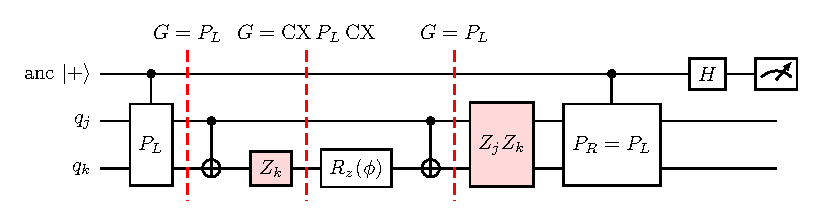
\includegraphics[width=0.85\textwidth]{figs/fig_zz_check.pdf}
\caption{One bond of the ZZ layer, $U=CX(j,k)R_z^{(k)}(\phi)CX(j,k)=\exp(-i\frac\phi2Z_jZ_k)$, bracketed by a coherent Pauli check. Dashed slices show the check image $G$ propagated to each time; the shaded boxes are the two faults that no valid flavor can see.}
\label{fig:zz}
\end{figure}

Split the window at a fault, $U=U_2EU_1$. Before the final Hadamard the joint state is $\tfrac1{\sqrt2}(|0\rangle\otimes U_2EU_1|\psi\rangle+|1\rangle\otimes P_RU_2EU_1P_L|\psi\rangle)$. With the check image at the fault location $G\equiv U_1P_LU_1^\dagger$ and $P_R=UP_LU^\dagger$,
\begin{equation}
P_RU_2EU_1P_L=U_2\,G\,E\,U_1P_L=U_2\,GEG\,U_1=\pm U_2EU_1,
\end{equation}
so the ancilla reads $1$ iff $E$ anticommutes with $G$, deterministically and independently of the data state. If the window contains $R_Q(\phi)$ and $G$ anticommutes with $Q$ there, then $R_QGR_Q^\dagger=\cos\phi\,G+i\sin\phi\,GQ$ is not a Pauli: no $P_R$ exists, and using the Clifford-propagated image instead makes the noiseless circuit flag with a state-dependent probability $\propto\sin^2\phi$. Validity therefore requires $[G,Q]=0$ at the rotation. For the gadget of Fig.~\ref{fig:zz} the rotation is $R_z$ on $q_k$ after the first CX, where $G=CX\,P_LCX$, and
\begin{equation}
[CX\,P_LCX,\ Z_k]=CX\,[P_L,\ CX\,Z_kCX]\,CX=CX\,[P_L,\ Z_jZ_k]\,CX,
\end{equation}
so $P_L$ must commute with $Z_jZ_k$, as expected from $U=\exp(-i\frac\phi2Z_jZ_k)$; then $P_R=P_L$.

Now apply the flag rule to the two shaded faults. For $Z_jZ_k$ after the second CX, $U_1=U$ and $G=UP_LU^\dagger=P_L$, which commutes with $Z_jZ_k$ by validity: flag $0$ for every valid $P_L$. For $Z_k$ after the first CX, $G=CX\,P_LCX$ and the commutator above vanishes by the same condition: flag $0$ again. Validity at the rotation and blindness to these two faults are the same condition. Physically, $Z_k$ between the two CX gates is an angle error, $CX\,Z_kR_z^{(k)}(\phi)\,CX\propto\exp(-i\frac{\phi+\pi}2Z_jZ_k)$, a $\pi$ over-rotation of the ZZ gate, and $Z_jZ_k$ after the gadget is the same over-rotation at the output; a check transparent to $\exp(-i\frac\phi2Z_jZ_k)$ for the programmed $\phi$ is transparent for every $\phi$ and cannot tell $\phi$ from $\phi+\pi$. In code language, the generator of a rotation that passes through the checks must be an undetectable operator of the detecting code, and errors along it are undetectable by definition. Every other Pauli fault at these locations has a back-propagated image with an $X$ or $Y$ component, or an odd Z-weight, and is flagged with probability exactly $\tfrac12$ under the twirl (Table~\ref{tab:fifteen}). The sector is therefore exactly one Pauli per CX location, which is why first-order PEC on it is cheap. Seeing it would require a check whose window ends between the first CX and the $R_z$, i.e.\ two check pairs per bond per step, or equivalently cutting the check at the rotation with controlled-$V$ gates; both cost more gadget gates than the payload. A native $R_{ZZ}$ gate has the same single invisible Pauli, $Z_jZ_k$.

\begin{table}[h]
\centering\small
\caption{Flag probability of the 15 two-qubit Pauli faults after the first CX of Fig.~\ref{fig:zz} (first letter on $q_j$, second on $q_k$), via the back-propagated image $Q=CX\,E\,CX$, for the two flavor families and their $\tfrac12$--$\tfrac12$ mixture.}
\label{tab:fifteen}
\begin{tabular}{p{4.2cm}lccc}
\toprule
fault $E$ & image $Q$ & Z-string & XY-string & mixture \\
\midrule
IX, IY, XI, XX, XY, XZ, YI, YX, YY, YZ, ZX, ZY & has $X$ or $Y$ & $\tfrac12$ & $\tfrac12$ & $\tfrac12$ \\
ZI, ZZ & ZI, IZ (odd Z-weight) & 0 & 1 & $\tfrac12$ \\
IZ & ZZ (even Z-weight) & 0 & 0 & 0 \\
\bottomrule
\end{tabular}
\end{table}

\paragraph{Catching it anyway: the controlled-$V$ repair.} The constraint on the flavor, not the rotation, hides the fault, and the repair of Martiel and Javadi-Abhari (SI \S V.B) removes the constraint. Allow any $P_L$; for every bond whose $Z_jZ_k$ anticommutes with $P_L$, insert controlled-$X_k$ from the same ancilla immediately before and after the $R_z$. In the ancilla-$|1\rangle$ branch the sandwich reverses the rotation, $X_kR_z(\phi)X_k=R_z(-\phi)$, and $P_L\,ZZ(-\phi)=ZZ(\phi)\,P_L$ for anticommuting $P_L$, so the branch equals $\pm$ the other one and $P_R=P_L$ stays valid. Now $Z_k$ after CX\#1 sits before the sandwich where the image is $CX\,P_LCX$, and $Z_jZ_k$ after CX\#2 meets the image $P_L$; both anticommute for half of all flavors. With $P_L$ uniform over all $4^n$ Paulis every payload fault is a fair coin, and the only invisible fault is a $Z_k$ between the two controlled-$X$ gates, an error of the (virtual) $R_z$ itself. The cost is two extra two-qubit gates per anticommuting bond, on average $n$ per step, so 12.5 gadget gates per step against 7.5 for the constrained family and 10 for the payload. Section~\ref{sec:demo} tests it.

A window containing an $R_x$ layer admits only X-strings, and a window spanning both layers admits only the global parity $\prod_iX_i$. Twirled checks on this circuit are therefore one per ZZ layer, with disjoint windows, and the threshold stratification (\ref{eq:threshold}) is the matching analysis.

\section{Relation to Pauli-path reactivity functions}
\label{sec:reactivity}

Expanding the observable in Pauli paths and grouping paths by their noise exposure $v$ gives $C=\sum_ve^{-v}R(v)$ with the reactivity function $R(v)$; rate scaling by $G$ gives $C(G)=\sum_ve^{-Gv}R(v)$, and any linear estimator $\hat C=\sum_rh_rC(G_r)$ acts as a filter, $\hat C=\sum_ve^{-v}h(v)R(v)$, with bias $\sum_v[1-e^{-v}h(v)]R(v)$ and cost $(\sum|h|)^2$ (Suchsland \emph{et al.}, arXiv:2609.31934). Probabilistic error cancellation is the filter $h=e^{v}$ at cost $e^{4\Lambda}$; Richardson extrapolation matches $e^{v}$ to a finite order in $v$.

In this language post-selection on twirled checks with full visibility is the filter $e^{-v}h_\acc(v)=(1-u)+ue^{-v}$: it does not act on exposures but mixes in the undamped reactivity. The leak subtraction (\ref{eq:leak}) has $e^{-v}h\equiv1$, the PEC filter, at cost $1/\alpha\approx e^{\Lambda_\vis}$ instead of $e^{4\Lambda}$: PEC isolates the zero-fault sector by signed interference of insertion experiments, a twirled check tags every nonzero net fault with a fair coin and the subtraction removes the tagged fraction by counting. For fixed checks the post-selected signal is a two-variable reactivity $R(v_d,v_u)$ in the detected and undetected exposures, and the ratio $r$ of (\ref{eq:two-point}) is its first-order cumulant; the failure of the first-order ratio on non-Clifford circuits and the success of a ratio fitted on Clifford training circuits are the statements that the second cumulants matter and that a fitted coefficient absorbs them. Per-fault heralded detection, finally, rescales every rate by $\sigma<1$ and is the ordinary exponential family entered from below; with the same ansatz, data at $G<1$ instead of $G>1$ reduced the zero-noise extrapolation bias by $4$--$40\times$ in our Ising tests.

\section{Numerical verification on Clifford circuits}
\label{sec:clifford}

All statements of Secs.~\ref{sec:twirl}--\ref{sec:species} were checked exactly on a 10-qubit random Clifford brickwork payload (50 CZ gates) with a stabilizer observable of ideal value 1, using the detector error model of \texttt{stim} and a Walsh--Hadamard transform to obtain the joint distribution of syndrome and observable flip at infinite shots, pooled over $M$ independent flavor draws.

\begin{table}[h]
\centering\small
\caption{Mixture law with six full-weight twirled checks, two-qubit depolarizing noise $p=0.004$ on every payload gate, noiseless gadgets, $M=1000$ flavor draws. $u=2^{-m}/\alpha_m$; estimator (\ref{eq:leak}).}
\label{tab:cliff}
\begin{tabular}{cccccc}
\toprule
$m$ & $\alpha_m$ & $u$ & $O_\PS$ & $\hat O_\varnothing$ \\
\midrule
0 & 1.0000 & 1.0000 & 0.8321 & --- \\
1 & 0.9093 & 0.5499 & 0.9076 & 0.9999 \\
2 & 0.8637 & 0.2894 & 0.9516 & 1.0003 \\
3 & 0.8411 & 0.1486 & 0.9751 & 1.0000 \\
4 & 0.8297 & 0.0753 & 0.9875 & 1.0001 \\
6 & 0.8213 & 0.0190 & 0.9968 & 1.0000 \\
\bottomrule
\end{tabular}
\end{table}

\begin{figure}[h]
\centering
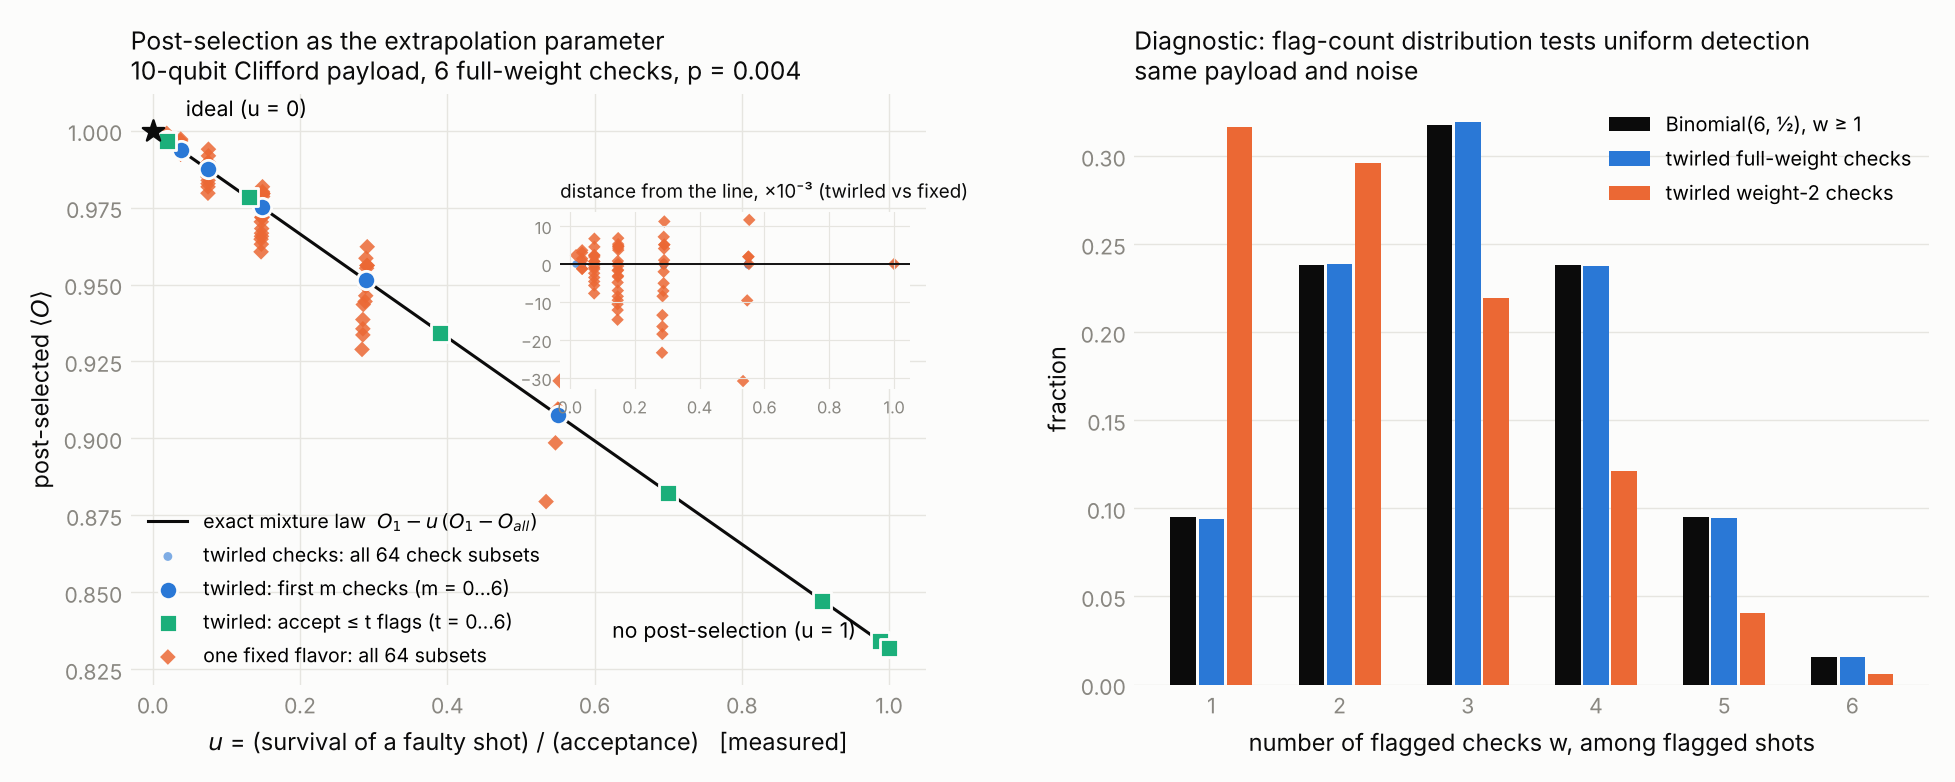
\includegraphics[width=\textwidth]{figs/fig_theory_mixture.png}
\caption{Left: post-selected $\langle O\rangle$ against the measured $u$ for six full-weight checks. With twirled flavors the first-$m$-checks family, the flag-threshold family and all 64 check subsets lie on the line $O_\varnothing-u(O_\varnothing-O_\all)$ (inset: residuals $\times10^{3}$); with one fixed flavor the 64 subsets scatter by up to $\pm2\%$. Right: the flag-count distribution among flagged shots is $\Bin(6,\tfrac12)$ for twirled full-weight checks and not for twirled weight-2 checks, whose faults are seen by varying numbers of checks.}
\label{fig:mixture}
\end{figure}

Further checks (all with residuals at the $10^{-3}$ level set by the finite number of flavor draws): threshold rules $t=0,\dots,5$; readout error $3\%$ (no effect); three times the noise; biased random per-location Pauli rates with $Z$-type faults four times heavier plus a correlated three-qubit fault per layer, at $p=0.004$ and $p=0.012$. With one fixed flavor the same estimator wanders between $0.981$ and $1.004$ across subset sizes. Three twirled weight-2 checks on distinct supports give single-species estimates between $0.924$ and $0.964$ depending on the subset and a stratified value of $0.998$. With noisy gadgets ($p_{\rm check}=p$) the single-species estimate acquires a multiplicity bias of up to $4\%$ for six checks, because faults in the right gadget of check $j$ are seen only by the checks outside it; nested stratification brings it back to $10^{-3}$ for depolarizing and biased gadget noise alike, with or without $1\%$ readout error.

\section{Comparison on a deep Trotter circuit}
\label{sec:demo}

\subsection{Setup}

The circuit is a transverse-field Ising ring of $n=5$ qubits in $|+\rangle^{\otimes5}$. One Trotter step applies $R_x(\theta)$ on every qubit and then one ZZ layer in which every bond $(j,k)$ receives $\exp(-i\tfrac\phi2Z_jZ_k)$ compiled as $CX(j,k)R_z^{(k)}(\phi)CX(j,k)$, bonds ordered even, odd, closing; $\theta=3\pi/8$, $\phi=-\pi/4$. Depths $d=2,\dots,16$ give 20 to 160 CX gates. The observable is the mean magnetization $m_x=\tfrac15\sum_i\langle X_i\rangle$, whose ideal value oscillates with depth (0.64, 0.49, 0.84, 0.65, 0.52, 0.94, 0.81, 0.43).

Noise: two-qubit depolarizing noise of total probability $p=0.01$ after every CX and after every controlled-Pauli of a check gadget, readout flip $q=0.01$ on the check ancilla, perfect single-qubit gates and resets. The state is evolved exactly as a density matrix; for checked circuits it is branched by the number of flagged checks, so every threshold rule is evaluated exactly. Finite-shot experiments ($N=10^4$ shots, 300 repetitions) are sampled from the exact X-basis outcome distributions of the branches; in the twirled protocol every shot draws its own flavor from a pool of 200 pre-computed draws. The RMSE is $\sqrt{\text{bias}^2+\text{std}^2}$ and the number of shots to reach RMSE $\le\varepsilon$ is $N_{\rm req}=N\Var/(\varepsilon^2-\text{bias}^2)$, infinite when the bias exceeds $\varepsilon$.

\subsection{Protocols}

\paragraph{Stage 1: zero-noise extrapolation.} No checks. All CX rates are scaled exactly by $G=1,2,3$ (the best case for ZNE). Exponential fit through $G=1,2$, and second-order cumulant fit (quadratic in $G$ for $\ln m_x$) through $G=1,2,3$; shots split equally across gains.

\paragraph{Stage 2: fixed Pauli checks, full post-selection.} One ancilla per Trotter step brackets the ZZ layer with the fixed flavor $X^{\otimes5}$ (equivalently $Z^{\otimes5}$), which flags a fault iff it has an odd number of $Y$ or $Z$ components, 8 of the 15 two-qubit Paulis, deterministically. Accept only shots with no flag. Two references complete this stage in the spirit of error detection plus first-order PEC on the undetected faults: an \emph{optimistic} one with noiseless gadgets and the undetected payload faults cancelled exactly (cost $e^{4\Lambda_u}/\alpha$), and a \emph{realistic} one with noisy, unmitigated gadgets.

\paragraph{Stage 3: twirled checks, partial post-selection, stratified extrapolation.} Same ancilla and windows; the flavor is redrawn for every shot from the family of Sec.~\ref{sec:nonclifford} (gadget cost 10 controlled-Paulis for an XY-string, 2.5 on average for a Z-string). All $d+1$ threshold rules are evaluated on the same shots and the species $f\le5$ are recovered from (\ref{eq:threshold}) by least squares; the estimate is $W_0/q_0$. ``PS only'' (no flags, no extrapolation) and the single-species leak subtraction with $\beta=\tfrac12$ are reported for comparison. This is the model-free core of the protocol: it removes exactly the faults the checks can see. Variant 3b adds first-order PEC on the invisible sector, and we regard the three-part pipeline (twirl, stratified extrapolation, PEC on the invisible sector) as the protocol proper, with the explicit statement that its only model input is one rate per gate. Variant 3c, the repaired full twirl described below, replaces the PEC step by a circuit modification and needs no model.

\paragraph{The PEC step on the invisible sector.} For the gadget $CX(j,k)R_z^{(k)}(\phi)CX(j,k)$ the faults invisible to every valid flavor are $Z_k$ after the first CX and $Z_jZ_k$ after the second (Sec.~\ref{sec:nonclifford}), both $\pi$ kicks of the ZZ angle, with rate $p/15$ each under depolarizing noise. In the simulation these two rates are set to zero exactly, which is the infinite-shot expectation of first-order PEC with exact rates, and the variance is multiplied by the PEC cost $\gamma^2=e^{4\Lambda_\inv}$ with $\Lambda_\inv=2\,(p/15)\times(\text{bonds})\times d$, i.e.\ $1.05$--$1.5$. In an experiment the two rates per CX location would be learned by sparse Pauli--Lindblad learning of the twirled CX layer (repeated-layer Pauli fidelities fitted to rates); the checks cannot supply them, since these faults never flag, and the $Z_k$, $Z_jZ_k$ rates lie near the known fidelity degeneracy of CX layers, which must be broken as in Chen \emph{et al.} (anchor paper, Ref.~9). PEC is then applied by quasi-probability sampling: at each location the Pauli is inserted with probability $\simeq\lambda_\nu$ and the sign of the shot flipped, and every outcome is weighted by $\gamma=\exp(2\sum_\inv\lambda_\nu)$. The inserted Paulis are even-weight Z-strings and therefore invisible to every flavor, so the flag statistics and the acceptance are unchanged and the post-selection probability is preserved, as the anchor paper's rescaling requires. The weighted outcomes enter the same stratified inversion, which is linear in the accepted sums, so the PEC weighting and the species inversion commute. Model error $\delta\Lambda_\inv$ in the learned rates enters as a bias of order $2\delta\Lambda_\inv$.

\paragraph{Stage 3c: repaired full twirl, any flavor $P_L$.} Same ancilla and windows, but $P_L$ is drawn uniformly from all $4^5$ Paulis, identity included, and the controlled-$X$ repair of Sec.~\ref{sec:nonclifford} is applied: for every bond whose $Z_jZ_k$ anticommutes with $P_L$, a controlled-$X_k$ from the same ancilla is inserted immediately before and after $R_z^{(k)}(\phi)$. In the ancilla-$|1\rangle$ branch the sandwich reverses the rotation, $X_kR_z(\phi)X_k=R_z(-\phi)$, and $P_L\,e^{+i\frac\phi2Z_jZ_k}=e^{-i\frac\phi2Z_jZ_k}P_L$ for anticommuting $P_L$, so the two branches agree up to a sign and $P_R=P_L$ remains a valid check. The flag rule of Sec.~\ref{sec:nonclifford} is unchanged, but the images met by the rotation-axis faults are now unconstrained: $Z_k$ after the first CX meets $CX\,P_L\,CX$ and $Z_jZ_k$ after the second meets $P_L$, each of which anticommutes with exactly half of all flavors. Every payload fault is therefore a fair coin (verified numerically: flag probabilities $0.49$, $0.49$, $0.49$ for $Z_k$, $Z_jZ_k$, $X_j$ over 4000 draws), there is no invisible sector, and the threshold-species inversion of Stage~3 applies as it stands, without PEC. The controlled-$X$ gates carry the same two-qubit depolarizing noise as the controlled-Paulis. On average half of the five bonds anticommute with a uniform flavor, so the gadget costs $7.5+5.0=12.5$ noisy two-qubit gates per step, against $7.5$ for the constrained family and $10$ for the payload. Species $f\le7$ are used, because the extra gadget noise raises the typical number of faulty steps: with $f\le5$ a truncation bias of $+0.02$ appears at depth 12, while $f\le6$ and $f\le7$ agree to $2\times10^{-3}$. Shots, repetitions and the flavor pool are as in Stage~3.

\paragraph{ED+PEC in detail.} The anchor paper's protocol is: learn a sparse Pauli--Lindblad model of every unique layer, payload and gadgets; back-propagate the check operators to classify each elementary fault as detected or undetected; use that individually undetected faults keep their generator exactly, so that to first order the post-selected logical noise is $\calL_u=\sum_{\nu\in V_u}\lambda_\nu(\calP_\nu-1)$ (detected faults enter only through syndrome-cancelling pairs at second order); invert $e^{-\calL_u}$ by PEC with weight $\gamma_L=\exp(2\sum_{V_u}\lambda_\nu)$; post-select on the trivial syndrome with the unnormalized-mean rescaling, which for equal shot counts is pooling. The cost is $\Gamma=\gamma_L^2/\alpha$. Our reference implements this for the fixed flavor $X^{\otimes5}$: at each CX location the 15 Paulis are classified deterministically (back-propagating through the first CX for faults after it), 7 of 15 are undetected, their rates are set to zero (the PEC expectation with exact rates), and the cost $e^{4\Lambda_u}/\alpha$ with $\Lambda_u=14\,(p/15)\times5\times d$ is charged to the variance as $N\Var\simeq(\gamma^2-O^2)/\alpha$. The \emph{optimistic} version has noiseless gadgets, equivalent to assuming that the gadget faults are learned and cancelled at no cost: an upper bound on accuracy and a lower bound on cost. The \emph{realistic} version leaves the gadget noise in place and unmitigated. The actual protocol lies between: the gadget faults would be in the learned model, their undetected part adds to $\Lambda_u$ and their detected part lowers $\alpha$. With a gadget weight of $0.1\,d$ and about half of it undetected, $\gamma^2$ grows by roughly $e^{0.2d}$, a factor of about 11 at $d=12$, which would place the realistic ED+PEC cost at or above that of the twirled protocol. This estimate is rough; the exact classification of ancilla-involving gadget faults for a fixed check has not been carried out.

\subsection{Results}

\begin{table}[h]
\centering\small
\caption{Infinite-shot bias of $m_x$.}
\label{tab:bias}
\setlength{\tabcolsep}{4pt}
\begin{tabular}{lrrrrrrrr}
\toprule
protocol & $d{=}2$ & 4 & 6 & 8 & 10 & 12 & 14 & 16 \\
\midrule
raw & $-0.061$ & $-0.070$ & $-0.247$ & $-0.219$ & $-0.183$ & $-0.486$ & $-0.448$ & $-0.191$ \\
ZNE exponential & $+0.001$ & $+0.006$ & $-0.004$ & $+0.002$ & $+0.015$ & $-0.028$ & $-0.020$ & $+0.056$ \\
ZNE 2nd cumulant & $0.000$ & $+0.001$ & $-0.001$ & $0.000$ & $+0.004$ & $-0.008$ & $-0.009$ & $+0.028$ \\
fixed checks, full PS & $-0.055$ & $-0.062$ & $-0.226$ & $-0.199$ & $-0.166$ & $-0.455$ & $-0.419$ & $-0.173$ \\
ED+PEC, optimistic & $-0.002$ & $-0.002$ & $-0.007$ & $-0.006$ & $-0.006$ & $-0.015$ & $-0.015$ & $-0.006$ \\
ED+PEC, realistic & $-0.025$ & $-0.022$ & $-0.120$ & $-0.099$ & $-0.072$ & $-0.266$ & $-0.241$ & $-0.064$ \\
twirled, PS only & $-0.061$ & $-0.071$ & $-0.240$ & $-0.216$ & $-0.182$ & $-0.474$ & $-0.439$ & $-0.192$ \\
twirled, stratified & $-0.008$ & $-0.010$ & $-0.025$ & $-0.030$ & $-0.029$ & $-0.064$ & $-0.055$ & $-0.026$ \\
twirled, stratified + PEC(inv) & $-0.001$ & $+0.001$ & $0.000$ & $-0.003$ & $-0.001$ & $-0.009$ & $+0.002$ & $+0.013$ \\
repaired full twirl (3c) & $0.000$ & $0.000$ & $-0.001$ & $-0.001$ & $0.000$ & $-0.002$ & $-0.001$ & $+0.003$ \\
\bottomrule
\end{tabular}
\end{table}

\begin{table}[h]
\centering\small
\caption{Standard deviation of $m_x$ at $10^4$ shots (300 repetitions).}
\label{tab:std}
\begin{tabular}{lrrrrrrrr}
\toprule
protocol & $d{=}2$ & 4 & 6 & 8 & 10 & 12 & 14 & 16 \\
\midrule
ZNE exponential & 0.020 & 0.024 & 0.029 & 0.033 & 0.032 & 0.047 & 0.055 & 0.050 \\
ZNE 2nd cumulant & 0.039 & 0.052 & 0.069 & 0.079 & 0.082 & 0.143 & 0.167 & 0.176 \\
fixed checks, full PS & 0.005 & 0.006 & 0.007 & 0.008 & 0.008 & 0.010 & 0.011 & 0.011 \\
ED+PEC, optimistic & 0.011 & 0.016 & 0.019 & 0.026 & 0.034 & 0.042 & 0.056 & 0.073 \\
twirled, stratified & 0.006 & 0.011 & 0.020 & 0.029 & 0.040 & 0.080 & 0.123 & 0.135 \\
twirled, stratified + PEC(inv) & 0.007 & 0.011 & 0.021 & 0.032 & 0.045 & 0.094 & 0.149 & 0.167 \\
repaired full twirl (3c) & 0.008 & 0.015 & 0.032 & 0.049 & 0.075 & 0.226 & 2.02 & 8.15 \\
\bottomrule
\end{tabular}
\end{table}

\begin{table}[h]
\centering\small
\caption{Shots (before post-selection) needed for RMSE $\le0.02$. $\infty$: bias exceeds the target.}
\label{tab:shots}
\begin{tabular}{lrrrrrrrr}
\toprule
protocol & $d{=}2$ & 4 & 6 & 8 & 10 & 12 & 14 & 16 \\
\midrule
ZNE exponential & 9k & 15k & 22k & 27k & 55k & $\infty$ & 5.1M & $\infty$ \\
ZNE 2nd cumulant & 38k & 69k & 121k & 158k & 174k & 615k & 849k & $\infty$ \\
fixed checks, full PS & $\infty$ & $\infty$ & $\infty$ & $\infty$ & $\infty$ & $\infty$ & $\infty$ & $\infty$ \\
ED+PEC, optimistic & 3k & 6k & 10k & 18k & 31k & 105k & 169k & 147k \\
twirled, stratified & 1k & 4k & $\infty$ & $\infty$ & $\infty$ & $\infty$ & $\infty$ & $\infty$ \\
twirled, stratified + PEC(inv) & 1k & 3k & 11k & 26k & 51k & 277k & 556k & 1.2M \\
repaired full twirl (3c) & 2k & 6k & 26k & 61k & 140k & 1.3M & $1.0{\times}10^8$ & $1.7{\times}10^9$ \\
\bottomrule
\end{tabular}
\end{table}

Acceptance of the twirled protocol with no flags falls from 0.83 at $d=2$ to 0.23 at $d=16$; the inferred clean fraction $q_0$ from 0.71 to 0.06. Fixed-check acceptance falls from 0.80 to 0.17. For the repaired full twirl the no-flag acceptance falls from 0.79 to 0.15 and the clean fraction $q_0$ from 0.63 to 0.02 (0.63, 0.39, 0.25, 0.15, 0.10, 0.06, 0.04, 0.02), roughly the square of the constrained family's, as expected from a gadget 1.7 times noisier. The optimistic ED+PEC cost $e^{4\Lambda_u}/\alpha$ grows from 1.6 to 53.

\begin{figure}[h]
\centering
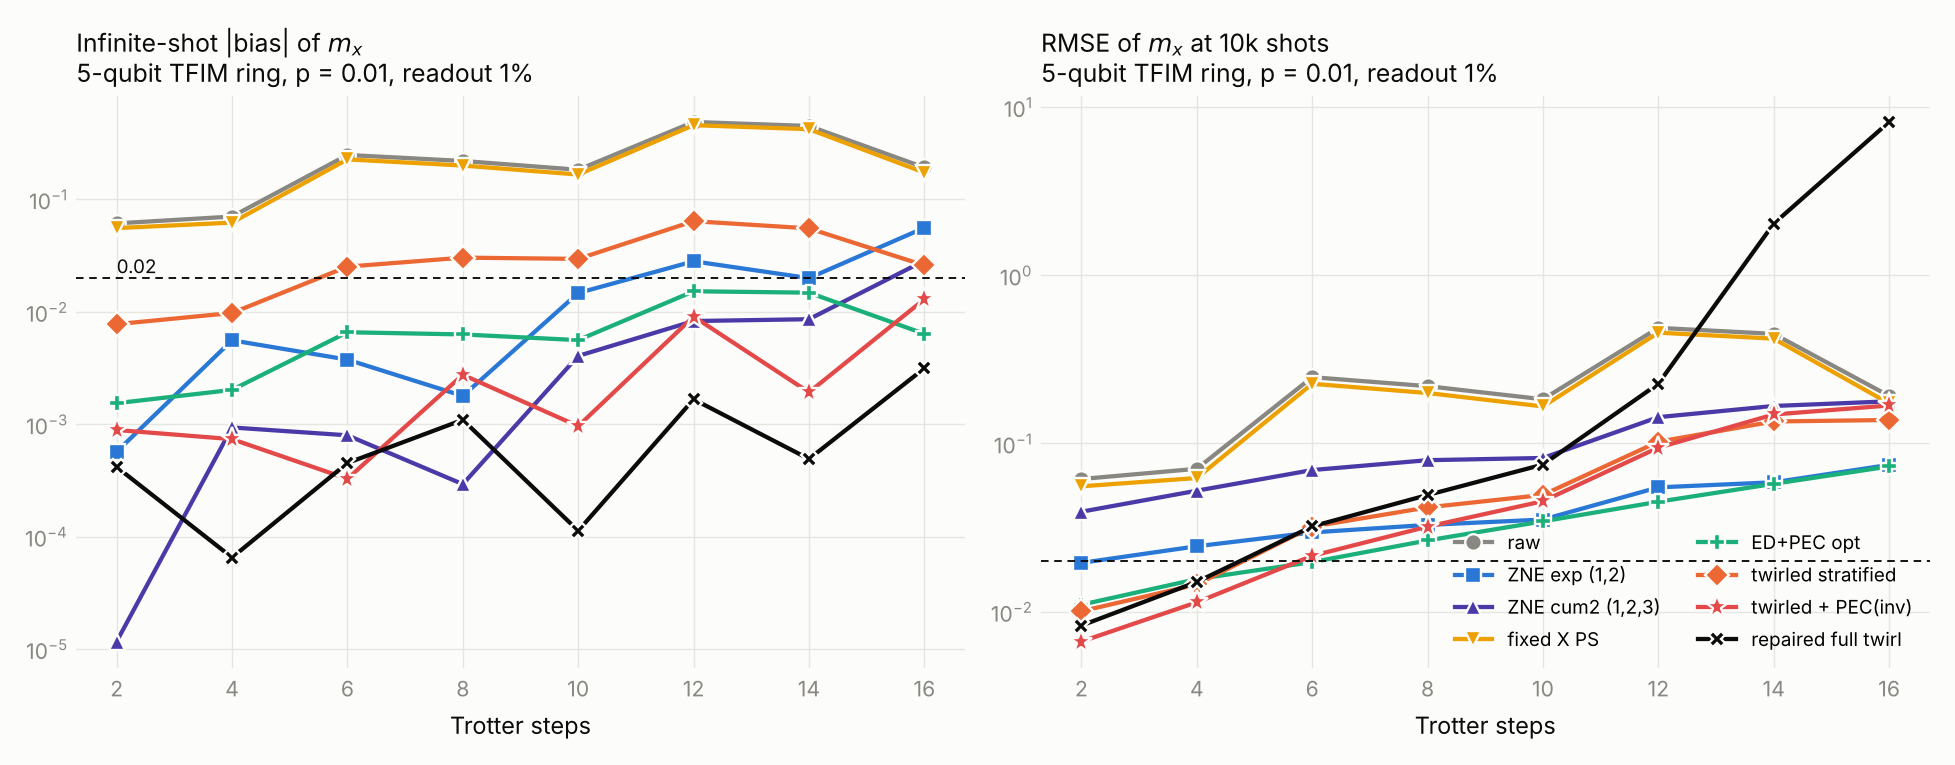
\includegraphics[width=\textwidth]{figs/fig_demo_bias_rmse.png}
\caption{Infinite-shot bias (left) and RMSE at $10^4$ shots (right) of $m_x$ against Trotter depth. Dashed line: the 0.02 target. Black crosses: the repaired full twirl (Stage 3c), with the smallest bias at every depth and the fastest-growing RMSE.}
\label{fig:bias}
\end{figure}

\begin{figure}[h]
\centering
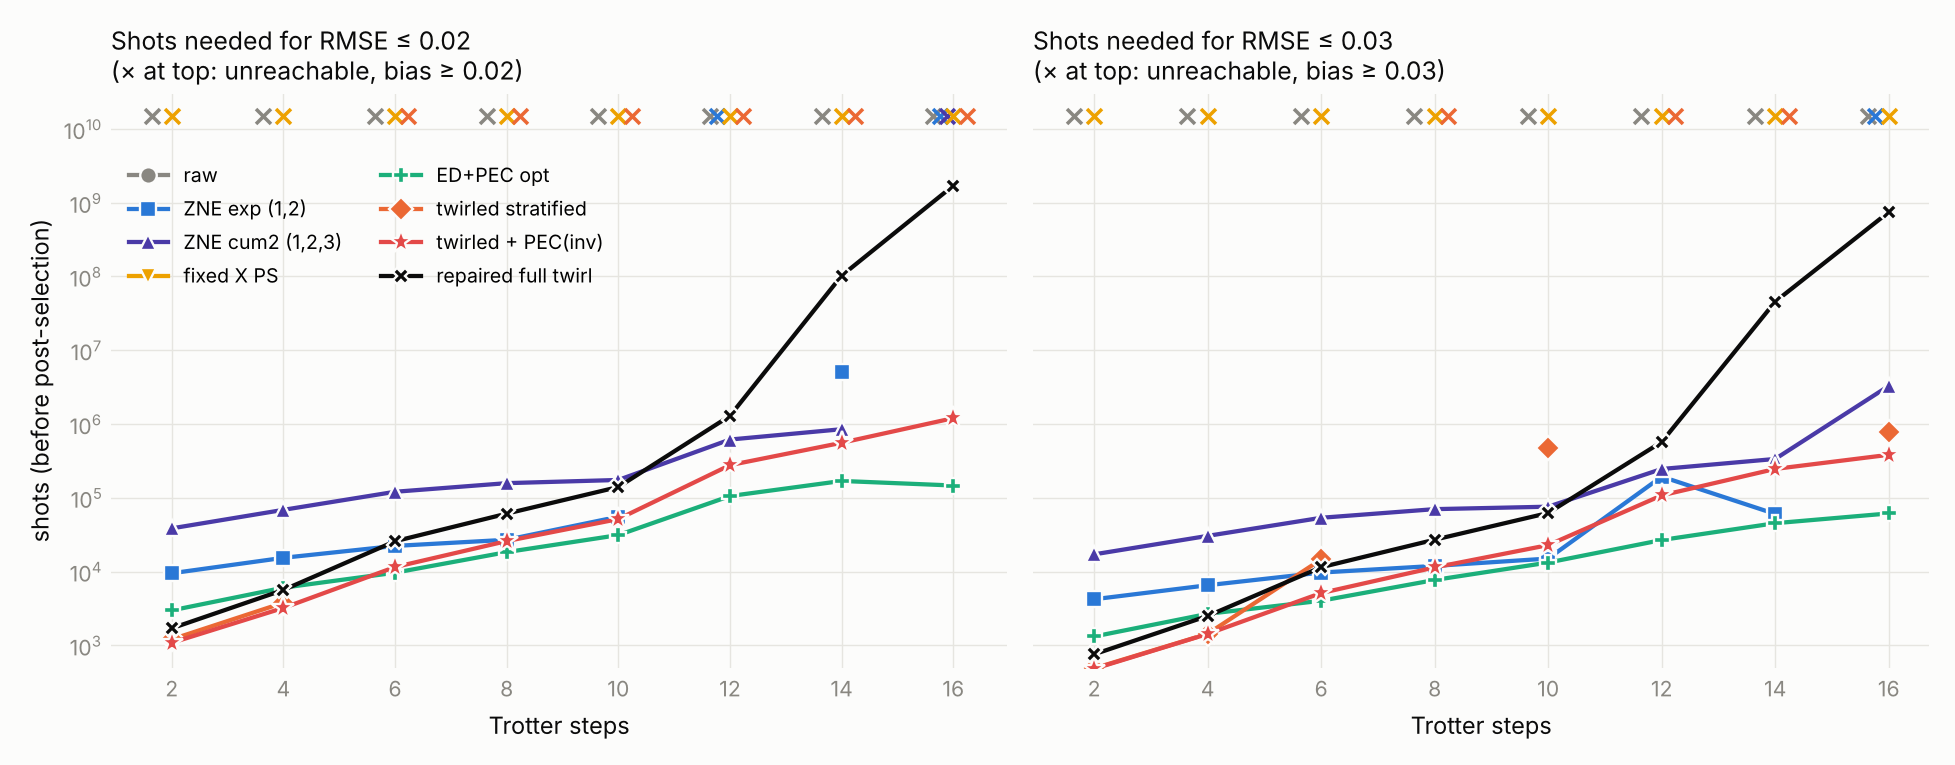
\includegraphics[width=\textwidth]{figs/fig_demo_shots.png}
\caption{Shots needed for RMSE $\le0.02$ (left) and $\le0.03$ (right). Crosses at the top mark protocols whose bias alone exceeds the target. The repaired full twirl reaches both targets at every depth but its shot count passes $10^8$ at depth 14.}
\label{fig:shots}
\end{figure}

\subsection{Discussion}

\paragraph{Zero-noise extrapolation.} On this observable the decay is close to a single exponential, so exponential ZNE is unbiased to about $0.01$ up to depth 10; what fails first is the variance, $0.02$--$0.05$ at $10^4$ shots, because the amplified points carry little signal. Beyond depth 10 the bias also exceeds $0.02$. The second-cumulant fit removes most of the bias and triples the scatter.

\paragraph{Fixed checks.} A fixed check removes about half of the payload noise deterministically and adds ten noisy gadget gates per step; the net effect on the bias is a few per cent, and no number of shots helps. The completion by first-order PEC on the undetected faults works and is the cheapest unbiased method in the table in its optimistic form; with the gadget noise left in, the bias is $0.02$--$0.27$. In practice the gadget noise would also be learned and cancelled, which raises $\Lambda_u$ and the cost; the optimistic line is a lower bound on the cost of that protocol.

\paragraph{Twirled checks.} Post-selection alone is useless, as Theorem~\ref{thm:mixture} predicts: each faulty step leaks with probability $\tfrac12$, so the accepted set is almost as noisy as the raw one. The extrapolation does the work. The single-species formula fails beyond depth 2 because most faulty shots have more than one faulty step; the threshold stratification handles this and is exact up to the invisible sector, whose residual ($0.01$--$0.06$) variant 3b removes. The variance of the stratified estimator grows roughly as $e^{\Lambda_{\rm total}}$ times an amplification of about 4 for isolating the clean species, which is why it overtakes the ZNE variance at depth 12. Weighted least squares does not reduce it, truncating at $f\le3$ adds bias, and two or three checks per step make the bias worse (depth 8: $-0.03\to-0.06$) because the additional gadget noise outweighs the sharper coin.

\paragraph{Repaired full twirl.} Allowing every flavor and repairing the anticommuting bonds with controlled-$X$ gates removes the invisible sector without any model, and Table~\ref{tab:bias} shows the result: $|{\rm bias}|\le0.002$ for $d\le14$ and $0.003$ at $d=16$, against $0.013$ for the PEC-completed constrained twirl and $0.056$ for exponential ZNE at $d=16$. It is the least biased protocol in the study and the only unbiased one that needs no noise information at all. Its price is the gadget noise. The clean fraction $q_0$ is roughly the square of the constrained family's, and the cost follows it: up to depth 10 the standard deviation is $1.2$--$1.7\times$ that of the constrained twirl with PEC and the shot count $2$--$3\times$ (2k, 6k, 26k, 61k, 140k for RMSE $\le0.02$); at depth 12 the ratios are $2.4\times$ and $5\times$ (1.3M shots); at depths 14 and 16, where $q_0<0.04$, the species inversion amplifies the shot noise by two orders of magnitude (standard deviation 2.0 and 8.1 at $10^4$ shots, formal shot counts $10^8$ and $2\times10^9$). The species cutoff is not the cause: at depth 12, $f\le5,6,7$ give standard deviations 0.24, 0.22, 0.23, and at depth 14, $f\le6$ and $7$ give 1.8 and 2.0. The amplification is the $1/(\alpha-\beta)^2$ of the leak-subtraction cost (\ref{eq:var}) compounded by the near-degeneracy of the threshold survival matrix (\ref{eq:threshold}) when the clean species is a few per cent of the accepted shots. The choice between 3b and 3c is therefore a choice between one learned rate per gate and five extra gadget gates per step: when the rotation-axis rate can be learned reliably the constrained family with PEC is $2$--$5\times$ cheaper and remains usable to depth 16; when the ZZ-type error is dominant or poorly characterized, which is common for two-qubit gates, the repair is the safe choice up to the depth at which $q_0$ falls below a few per cent. A flavor distribution that keeps the number of anticommuting bonds small while preserving the $\tfrac12$ coin for the rotation-axis faults would move the crossover to larger depth.

\paragraph{Comparison.} Against exponential ZNE the twirled protocol has smaller bias at every depth, needs fewer shots wherever both reach the target, and reaches it where ZNE cannot. Against second-cumulant ZNE it needs $2$--$30\times$ fewer shots. Against the optimistic model-based ED+PEC reference it is comparable up to depth 8 and $3$--$8\times$ more expensive beyond, while requiring one noise rate per gate instead of a full model of payload and gadgets. Fixed checks with full post-selection never reach the target. The repaired full twirl (3c) is the most accurate line at every depth and the most expensive one beyond depth 10 at $1\%$ error; Sec.~\ref{sec:threshold} shows that this ordering is a statement about the clean fraction, not about the protocol, and reverses once $q_0\gtrsim0.3$.

\subsection{Noise-level dependence and break-even}
\label{sec:threshold}

The repaired twirl is unbiased at every depth but, at $p=q=1\%$, the most expensive protocol beyond depth 10. To see whether this reverses as gates and readout improve, the comparison was repeated at $p=q=0.5\%$ ($d=12,16,20$) and $0.2\%$ ($d=16,24$), with exponential and second-cumulant ZNE at every point (100 flavor draws; otherwise as above). Table~\ref{tab:threshold} and Fig.~\ref{fig:threshold} give the result.

\begin{table}[h]
\centering\small
\caption{Noise-level scan: bias / standard deviation at $10^4$ shots / shots for RMSE $\le0.02$ of $m_x$. $q_0$ is the clean fraction of the repaired circuit.}
\label{tab:threshold}
\setlength{\tabcolsep}{3pt}\footnotesize
\begin{tabular}{llrllll}
\toprule
$p{=}q$ & $d$ & $q_0$ & ZNE exp. & ZNE 2nd cum. & twirled + PEC(inv) & repaired twirl \\
\midrule
1\% & 8 & 0.15 & $+0.002$ / 0.033 / 27k & $0.000$ / 0.079 / 158k & $-0.003$ / 0.032 / 26k & $-0.001$ / 0.049 / 61k \\
1\% & 12 & 0.06 & $-0.028$ / 0.047 / $\infty$ & $-0.008$ / 0.143 / 615k & $-0.009$ / 0.094 / 277k & $-0.002$ / 0.226 / 1.3M \\
1\% & 16 & 0.02 & $+0.056$ / 0.049 / $\infty$ & $+0.028$ / 0.176 / $\infty$ & $+0.013$ / 0.167 / 1.2M & $+0.003$ / 8.1 / $1.7{\times}10^9$ \\
0.5\% & 12 & 0.25 & $-0.008$ / 0.027 / 21k & $-0.001$ / 0.064 / 104k & $-0.002$ / 0.021 / 11k & $-0.001$ / 0.036 / 33k \\
0.5\% & 16 & 0.15 & $+0.020$ / 0.028 / 714k & $+0.007$ / 0.065 / 122k & $0.000$ / 0.027 / 18k & $0.000$ / 0.040 / 40k \\
0.5\% & 20 & 0.10 & $-0.012$ / 0.040 / 65k & $-0.003$ / 0.102 / 268k & $+0.001$ / 0.054 / 73k & $-0.002$ / 0.106 / 285k \\
0.2\% & 16 & 0.47 & $+0.004$ / 0.021 / 12k & $+0.001$ / 0.045 / 51k & $0.000$ / 0.009 / 2k & $0.000$ / 0.011 / 3k \\
0.2\% & 24 & 0.33 & $-0.003$ / 0.026 / 17k & $-0.001$ / 0.060 / 90k & $+0.001$ / 0.015 / 6k & $-0.001$ / 0.021 / 11k \\
\bottomrule
\end{tabular}
\end{table}

\begin{figure}[h]
\centering
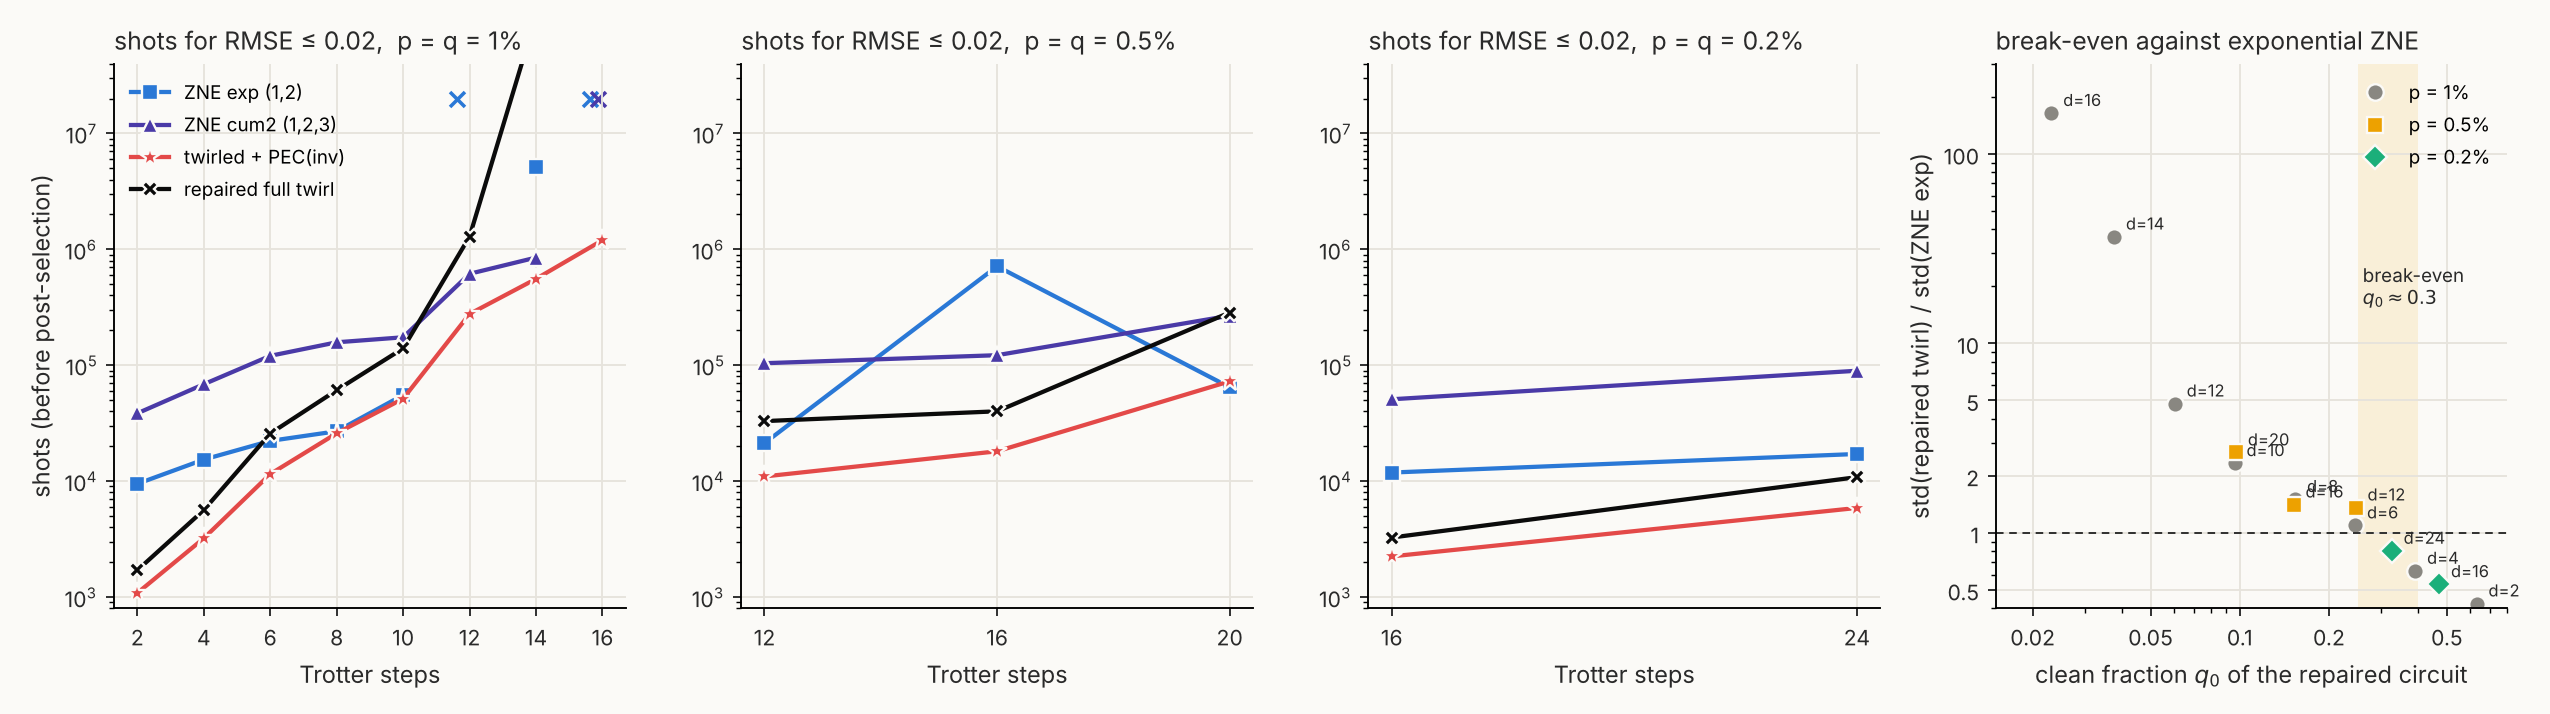
\includegraphics[width=\textwidth]{figs/fig_threshold.png}
\caption{Shots for RMSE $\le0.02$ against depth at $p=q=1\%$, $0.5\%$, $0.2\%$ (crosses at top: bias exceeds the target), and, right, the ratio of the repaired twirl's standard deviation to exponential ZNE's against the clean fraction $q_0$ of the repaired circuit for all noise levels and depths. The points collapse onto one curve with break-even at $q_0\approx0.3$.}
\label{fig:threshold}
\end{figure}

Three things follow. First, the bias of the check-based protocols does not depend on the noise level: the repaired twirl is within $0.003$ of the ideal at every point, and the constrained twirl with PEC within $0.003$ except at $1\%$, $d\ge12$, where the second-order remainder of the one-Pauli PEC appears. What moves is the bias of exponential ZNE, which exceeds $0.02$ at $1\%$ for $d\ge12$ and at $0.5\%$ for $d=16$ and is harmless at $0.2\%$. The checks never add error; the noise level decides only their cost.

Second, the cost ratio to ZNE is a function of the clean fraction alone. In the right panel of Fig.~\ref{fig:threshold} the points from all three noise levels lie on one curve: $\mathrm{std}_{\rm rep}/\mathrm{std}_{\rm ZNE}\approx1$ at $q_0\approx0.3$, $1.4$ at $0.15$, $2.5$ at $0.10$, $5$ at $0.06$, and divergent below $0.04$, where the inferred $q_0$ is within $3\sigma$ of zero at $10^4$ shots and the ratio estimator $W_0/\hat q_0$ becomes heavy-tailed. Pairs with equal $q_0$ at different $(p,d)$ agree: $(1\%,d{=}8)$ and $(0.5\%,d{=}16)$ have $q_0\approx0.15$ and ratios $1.49$ and $1.41$; $(1\%,d{=}10)$ and $(0.5\%,d{=}20)$ have $q_0\approx0.10$ and ratios $2.3$ and $2.7$.

Third, this fixes the constant in the break-even condition (\ref{eq:breakeven}) of Sec.~\ref{sec:breakeven}: with $q_0^\ast\approx0.3$ and (\ref{eq:q0}), detection-driven extrapolation is cheaper than exponential ZNE when
\begin{equation}
(g_p+g)\,p\,d\;\lesssim\;1.3 ,
\label{eq:threshold-cond}
\end{equation}
about one expected fault in the whole checked circuit, gadgets included. For the repaired gadget ($g_p+g=22.5$) this is $pd\lesssim0.06$: $d\lesssim6$ at $1\%$, $12$ at $0.5\%$, $29$ at $0.2\%$, $58$ at $0.1\%$; for the constrained family ($17.5$) $pd\lesssim0.075$. Where ZNE is biased the checks win regardless of cost, e.g.\ $0.5\%$, $d=16$: 714k shots for exponential ZNE against 40k (repaired) and 18k (constrained with PEC). At $0.2\%$ the repaired twirl is cheaper than exponential ZNE at every depth tested ($4\times$ at $d=16$, $1.6\times$ at $d=24$) with no noise model, and within $2\times$ of the constrained family with PEC.

The condition (\ref{eq:threshold-cond}) is the same bookkeeping as the critical payload error rate of van den Berg \emph{et al.} (PRR 2023), who find that coherent Pauli checks lower the logical error only when the payload error exceeds a critical value set by the check gadget's own gate count; here the extrapolation's amplification factor is included and the comparison is to ZNE rather than to the unmitigated circuit. The collapse onto $q_0$, the absence of a threshold in $p$ alone, and the asymptotic condition $1+r<G_{\max}\kappa$ are the content of Sec.~\ref{sec:breakeven}.

\section{Detection-conditioned extrapolation in error-detecting codes}
\label{sec:qed}

The twirled-check protocol of Secs.~\ref{sec:twirl}--\ref{sec:species} buys little on heavy-hex hardware (Appendix~\ref{app:hardware}): the checks cannot be twirled on mediated bonds and the gadgets cost as much as they remove. The same logic has a natural home in error-detecting codes, where the detectors exist anyway and the problem is the opposite one: full post-selection on trivial syndromes leaves no shots once the circuit is large, and the detector record is thrown away with them. This section shows that the detector count obeys an exact geometric law that turns post-selection into a regression over all shots, and says what it does not do. Details and the QEC extension are in \texttt{theory/qed\_extrapolation.md}.

\paragraph{Setting.} A Clifford code circuit with $K$ detectors (parities of measurement outcomes that are deterministic without faults) and a logical observable $O$ with outcome $o=\pm1$; a shot returns $(s,o)$, $s\in\{0,1\}^K$. Independent Pauli faults $\nu$ with rates $\lambda_\nu$; each fault has a syndrome $s_\nu$ (detected if $s_\nu\neq0$) and, by the Pauli-frame push-through, a logical effect $\epsilon_\nu=\pm1$ on $o$. Let $\Lambda_d$ be the detected weight, $\pi_d(\nu)=\lambda_\nu/\Lambda_d$, and $O_0=E[o\mid s=0]$ the fully post-selected value, which carries the undetected damage $e^{-2\Lambda_u^{(O)}}$; for a distance-2 code $\Lambda_u=O(\Lambda^2)$. Full post-selection keeps $N\alpha_0=Ne^{-\Lambda_d}$ shots.

\begin{theorem}[Geometric law]
\label{thm:geometric}
Let $k$ be the number of detected faults in a shot. Under independent Pauli faults in a Clifford circuit,
\begin{equation}
E[o\mid k]=O_0\,\bar\rho^{\,k},\qquad\bar\rho=E_{\pi_d}[\epsilon_\nu]=1-2\kappa_d,
\label{eq:geometric}
\end{equation}
with $\kappa_d$ the probability that a detected fault flips $O$.
\end{theorem}
\begin{proof}
Conditioned on $k$ detected faults, Poisson faults are $k$ iid draws from $\pi_d$, independent of the undetected configuration. Since $o=o_{\rm undet}\prod_{i\le k}\epsilon_{\nu_i}$, the expectation factorizes.
\end{proof}

The law is exact to all orders in the detected faults. $\ln E[o\mid k]$ is linear in $k$: the detection count is a noise meter and the observable follows one exponential in it. A weighted fit of $\ln\bar o_k$ against $k$ (or the two-parameter likelihood fit of $o_i$ with mean $O_0\bar\rho^{k_i}$) returns the fully post-selected value from every shot. With $\bar\rho$ known, a shot with $k$ detections carries Fisher weight $\bar\rho^{2k}$, so the effective shot count is
\begin{equation}
N_{\rm eff}=N\sum_kP(k)\bar\rho^{2k}=N\,\alpha_0^{\,1-\bar\rho^2},
\label{eq:neff}
\end{equation}
a gain of $\alpha_0^{-\bar\rho^2}=e^{\Lambda_d\bar\rho^2}$ over full post-selection. For a local logical observable in a large code most detected faults lie outside its light cone, $\kappa_d\ll1$ and $\bar\rho\approx1$: with $N=10^6$, $\alpha_0=10^{-3}$ and $\bar\rho=0.9$, full post-selection keeps $10^3$ shots and (\ref{eq:neff}) gives $2.7\times10^5$. In the language of Sec.~\ref{sec:fixed}, a code detector is a fixed check (coin 1 or 0), so post-selection is a projection and cannot be rescaled to the ideal value; what Theorem~\ref{thm:geometric} adds is that, with species labelled by the detected-fault count and iid damage per detected fault, the species contributions form a geometric sequence and the $k=0$ species is recoverable from all the others: it is the stratified inversion of Sec.~\ref{sec:species} with a one-parameter species model.

\paragraph{What the law does not do.} $O_0\neq O_{\rm ideal}$: the undetected sector is untouched by conditioning on $k$, by construction. Three routes remain. (a) \emph{ZNE from below with the detector as noise meter}: scale the noise by $G$; $\Lambda_d\to G\Lambda_d$ is \emph{measured} from the mean detection count, while $\Lambda_u^{(O)}\to G^2\Lambda_u^{(O)}$ for a distance-2 code, so $\ln O_0(G)=\ln O_{\rm ideal}-2G^2\Lambda_u^{(O)}$ is a one-parameter extrapolation in a quantity quadratic in the noise, with the achieved amplification read off the detectors rather than assumed. (b) \emph{Model-assisted}: $\Lambda_u^{(O)}=c\Lambda_d^2$ with $c$ a circuit property under an assumed noise shape and $\Lambda_d$ measured. (c) \emph{Learned rates}: the detector statistics determine the detected rates per location, the model gives the undetected ones, and first-order PEC on the undetected generator follows as in the anchor paper, from the same shots.

\paragraph{Detectors versus faults.} The law counts detected \emph{faults}. With a single terminal syndrome round of two stabilizers (Iceberg-style) the detectors report only parities, $k$ is hidden, and the $s=0$ bin is contaminated by even-$k$ cancellations with probability $\approx\Lambda_d^2/2$ per stabilizer: periodic syndrome checks are needed to make $k$ observable, which is a reason for them beyond detection itself. With periodic checks, $k$ is the number of fired windows up to a known second-order cancellation species; in surface-code-like detector lattices $k$ is the number of matched clusters.

\paragraph{Error-correcting codes.} For $d\ge3$ the decoder's soft output $g$ (the log-likelihood ratio of the chosen logical class, the complementary gap) gives the per-shot logical error probability $P_L(g)=1/(1+e^{g})$, and $E[o\mid g]=O_{\rm ideal}(1-2P_L(g))$: a regression of $o$ on the known function $1-2P_L(g)$ over all shots returns $O_{\rm ideal}$ with effective shot count $N\,E[(1-2P_L)^2]$ and no post-selection, unbiased to the extent that the decoder's likelihoods are calibrated, which the same data check (the disagreement rate at given $g$ must equal $P_L(g)$). This is Theorem~\ref{thm:geometric} with $\bar\rho^k$ replaced by the per-shot factor $1-2P_L(g)$.

\paragraph{Relation to Observable-Ranked Postselection.} The reference experiment for this setting (Froland \emph{et al.}, arXiv:2607.24947: 21 blocks of $[[4,2,2]]$ on ibm\_boston, Ising dynamics with non-fault-tolerant logical rotations and periodic syndrome extraction) meets the shot-loss problem with ORP: it computes $\Delta_j=E[Q\mid v_j{=}0]-E[Q\mid v_j{=}1]$ for every detector, ranks detectors by $\Delta_j$, keeps the shots in which none of the top-$k$ detectors fired, and picks $k^\ast$ by a plateau heuristic; at weak noise $\Delta_j\approx2\langle O\rangle\kappa_j$ with $\kappa_j$ the flip probability of the processes firing $v_j$, and the selected detectors lie in the backward light cone of $O$. Theorem~\ref{thm:geometric} applied detector by detector gives the exact form of what ORP measures,
\begin{equation}
E[Q\mid v]=O_0\prod_j\rho_j^{\,v_j},\qquad\rho_j=1-\frac{\Delta_j}{E[Q\mid v_j{=}0]}=1-2\kappa_j ,
\label{eq:loglinear}
\end{equation}
whose first-order expansion is the additive regression model ORP uses only as an alternative ranking. Fitting (\ref{eq:loglinear}) on all shots (two stages: $\rho_j$ from the detector-wise conditional means, then the weighted mean $\hat O_0=\sum_iw_iQ_i/\sum_iw_i^2$ with $w_i=\prod_j\rho_j^{v_{ij}}$) replaces the cut by a weight: detectors outside the light cone cost nothing, light-cone detectors down-weight a shot by $\rho_j^2$ instead of discarding it, there is no cut level to choose, and the linearity of $\ln E[Q\mid |v|{=}k]$ in $k$ is a built-in model check. The effective shot count is $N\exp[-\sum_jp_j(1-\rho_j^2)]$ against $N\exp[-\sum_{j\le k^\ast}p_j]$ for the cut, a gain of $\exp[\sum_jp_j\rho_j^2]$. The plateau level that ORP attributes to undetectable errors is $O_0$ here, and neither method reaches $O_{\rm ideal}$ without the second step. Since the estimator needs only the shot-level $(v_i,Q_i)$ records, it can be run on the existing data set; the expected outcome is the same central values with smaller error bars.

\paragraph{Assumptions.} Independent Pauli faults; a Clifford circuit, so that each fault's effect is a sign (for non-Clifford circuits the product structure holds only when the light cones of distinct detected faults do not overlap, and the law is then first order in the overlap probability); a detector count that resolves the fault count; and a separate treatment of the undetected sector. The first test is a \texttt{stim} simulation of a $[[4,2,2]]$ or $[[6,4,2]]$ circuit with periodic checks: linearity of $\ln E[o\mid k]$, the value of $\bar\rho$ against the fault enumeration, the variance of $\hat O_0$ against (\ref{eq:neff}), and the $G^2$ extrapolation with detector-measured gain.

\section{Limitations and open points}

\begin{itemize}
\item The invisible sector is intrinsic to checks compatible with the rotations; on this circuit it is 2 of 30 Pauli faults per bond gadget. It was removed either with a one-rate model-based correction (3b) or, model-free, by the controlled-$X$ repair (3c), whose extra gadget noise limits the usable depth. Learning that rate from the detection statistics, and a cheaper repair, are the natural next steps.
\item The variance of the stratified estimator carries a factor of about 4 from isolating the clean species in addition to $1/q_0$; a maximum-likelihood species fit and shot allocation across rules may reduce it.
\item The gadget cost of full-weight twirled checks (on average $\tfrac32n$ two-qubit gates per check) exceeds the payload cost per layer on small registers; Z-string flavors are four times cheaper than XY-strings, and a biased flavor distribution with the matching species model could halve the gadget noise.
\item The break-even (\ref{eq:breakeven}) was established against exponential ZNE on one observable; against second-cumulant ZNE the threshold sits lower, $q_0^\ast\approx0.1$, and against the optimistic model-exact ED+PEC reference, run only at $1\%$, the check-based extrapolation does not win on cost, only on model independence. No work in the Pauli-check literature states a break-even of this form; the closest is the critical payload error rate of van den Berg \emph{et al.}, which compares to the unmitigated circuit.
\item The ZNE baseline used exact rate scaling; probabilistic error amplification with a learned model would carry model error. The fixed-check baseline carried its gadget noise while the ED+PEC reference did not.
\item All numerics are at 5 to 10 qubits with independent Pauli noise, perfect resets and no leakage. The noise-level scan used 100 flavor draws and three noise levels; the collapse of the cost ratio onto a function of $q_0$ should be checked on other observables and circuits.
\end{itemize}

\appendix
\section{Check circuits used in the comparison}
\label{app:circuits}

Figures~\ref{fig:gadget-a}--\ref{fig:gadgets} draw the three circuits that enter the comparison of Secs.~\ref{sec:demo} and \ref{sec:threshold}: the payload step, the constrained twirled check used by the ``twirled stratified'' and ``twirled $+$ PEC(inv)'' lines, and the repaired full twirl. Table~\ref{tab:gadget-counts} collects the gate counts behind $g_p$ and $g$ in (\ref{eq:breakeven}).

\begin{figure}[h]
\centering
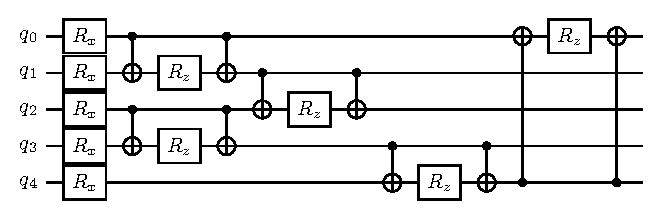
\includegraphics[width=0.8\textwidth]{figs/fig_gadget_a.pdf}
\caption{One Trotter step of the payload on the five-qubit ring: $R_x(\theta)$ on every qubit, then the ZZ layer with bonds $(0,1),(2,3)$, then $(1,2),(3,4)$, then the closing bond $(4,0)$, each compiled as $CX_{jk}R_z^{(k)}(\phi)CX_{jk}$; ten noisy CX gates per step ($g_p=10$).}
\label{fig:gadget-a}
\end{figure}

\begin{figure}[h]
\centering
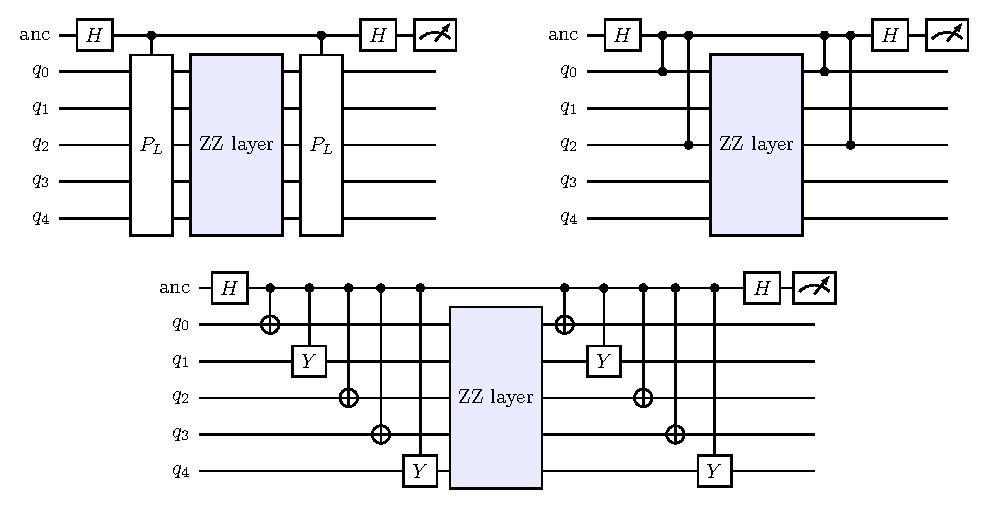
\includegraphics[width=0.9\textwidth]{figs/fig_gadget_b.pdf}
\caption{Constrained twirled check (lines ``twirled stratified'' and ``twirled $+$ PEC(inv)''). Ancilla prepared in $|+\rangle$, controlled-$P_L$ before the ZZ layer, controlled-$P_R=P_L$ after, Hadamard and measurement; flag $=1$ iff the net fault in the window anticommutes with the propagated image of $P_L$. Top left: generic form. The flavor is redrawn every shot from the family that commutes with every $Z_jZ_k$: with probability $\tfrac12$ a $Z$-string on a uniformly random subset (top right, $P_L=Z_0Z_2$: two controlled-$Z$ per side), with probability $\tfrac12$ a string with $X$ or $Y$ on every qubit (bottom, $P_L=X_0Y_1X_2X_3Y_4$: five controlled-Paulis per side). No repair gates; the two rotation-axis faults per bond are invisible and are handled by the one-Pauli PEC. Average gadget cost $g=7.5$ noisy two-qubit gates per step.}
\label{fig:gadget-b}
\end{figure}

\begin{figure}[h]
\centering
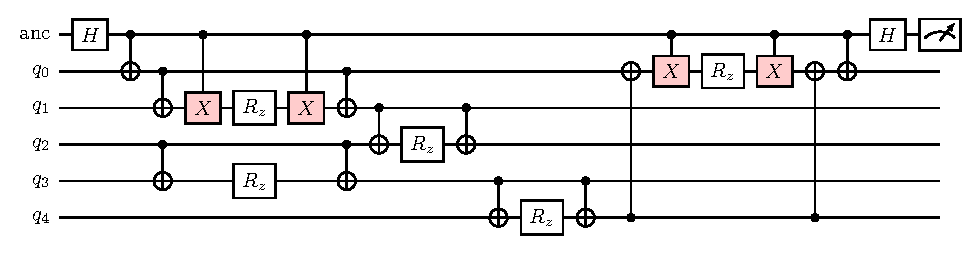
\includegraphics[width=\textwidth]{figs/fig_gadget_c.pdf}
\caption{Repaired full twirl (line ``repaired full twirl''). $P_L$ is uniform over all $4^5$ Paulis; for every bond whose $Z_jZ_k$ anticommutes with $P_L$ a controlled-$X_k$ from the same ancilla is placed immediately before and after $R_z^{(k)}$ (red), which reverses the rotation in the ancilla-$|1\rangle$ branch and keeps $P_R=P_L$ a valid check. Shown for $P_L=X_0$, which anticommutes with bonds $(0,1)$ and $(4,0)$, so the $R_z$ on $q_1$ and on $q_0$ are repaired. Every payload fault, the rotation-axis ones included, now flags with probability $\tfrac12$. Average gadget cost $g=7.5$ controlled-Paulis $+5.0$ controlled-$X$ $=12.5$ noisy two-qubit gates per step. In all three figures every two-qubit gate drawn carries the same depolarizing noise and the ancilla readout the flip probability $q$.}
\label{fig:gadgets}
\end{figure}

\begin{table}[h]
\centering\small
\caption{Noisy two-qubit gates per Trotter step and visibility of the payload faults for the two check protocols. Gadget counts are averages over the flavor distribution; a controlled-Pauli acts on one data qubit per non-identity letter of $P_L$, on both sides of the window.}
\label{tab:gadget-counts}
\begin{tabular}{lccc}
\toprule
 & payload $g_p$ & gadget $g$ & visible payload faults \\
\midrule
constrained twirled check (3, 3b) & 10 & $\tfrac12\cdot2\cdot5+\tfrac12\cdot2\cdot2.5=7.5$ & $13/15$ per CX location \\
repaired full twirl (3c) & 10 & $2\cdot3.75+2\cdot2.5=12.5$ & $14/15$ (all non-identity) \\
\bottomrule
\end{tabular}
\end{table}

For the constrained family, an XY-string has weight 5 on both sides (10 gates) and a $Z$-string on a uniform subset has mean weight $2.5$ on both sides (5 gates), so the average is $7.5$. For the repaired family, a uniform Pauli has a non-identity letter on each qubit with probability $\tfrac34$ (mean weight $3.75$ per side, $7.5$ controlled-Paulis), and each of the five bonds anticommutes with it with probability $\tfrac12$ (mean $2.5$ repaired bonds, $5$ controlled-$X$ gates), giving $12.5$. The two faults the constrained family cannot see are $Z_k$ between the two CX gates and $Z_jZ_k$ after the second (Sec.~\ref{sec:nonclifford}); in the repaired circuit both meet an unconstrained image and flag with probability $\tfrac12$, and the only fault that stays invisible is a $Z_k$ between the two red gates, an error of the virtual $R_z$ itself. The flag probability of every other fault is exactly $\tfrac12$ in both families (Table~\ref{tab:fifteen} and \texttt{demo/repaired.py}), which is what makes the species analysis of Sec.~\ref{sec:species} apply to both without modification. Sources: \texttt{paper/figs/fig\_gadget\_a.tex}, \texttt{\_b.tex}, \texttt{\_c.tex}.

\section{Hardware-native check circuits}
\label{app:hardware}

The gadgets of Appendix~\ref{app:circuits} apply controlled-Paulis from one ancilla to up to five data qubits and, in the repaired variant, controlled-$X$ gates to arbitrary bond targets. This assumes all-to-all ancilla--data connectivity. On a line or heavy-hex device a weight-$w$ controlled-Pauli from one ancilla costs about $3w$ CNOTs with routing (van den Berg \emph{et al.}, Table~1: $\approx9n/2$ two-sided on a line against $3n/2$ all-to-all), so the gadget counts $g=7.5$ and $12.5$ used in the main text are lower bounds by roughly a factor of three on hardware, and the $1\%$ results are optimistic for the check protocols. This appendix records how the spacetime-code papers place their checks, and a ring design that keeps the twirl with local gates only.

\paragraph{The anchor paper's implementation.} Fischer \emph{et al.} run the same TFIM dynamics on a heavy-hex device with 22 data qubits on the degree-3 sites and 27 ancillas on the degree-2 sites between them, one per bond. The bond interaction is implemented \emph{through} its ancilla, $CX_{j\to a}CX_{k\to a}R_z^{(a)}(\phi)CX_{k\to a}CX_{j\to a}$ (4~CZ per bond per step, 216 CZ for 27 bonds at $d=2$); the ancilla starts in $|0\rangle$, ideally returns to $|0\rangle$ after every step, is never measured mid-circuit, and its terminal $Z$ measurement is the check (Fig.~\ref{fig:hw-gadget}, left). Back-propagating $Z_a$ gives the image $Z_jZ_a$ after the first CX, $Z_jZ_kZ_a$ between the second and third, and $Z_a$ outside the gadget. Hence the check costs no extra two-qubit gate ($g=0$): the mediator that connectivity forces is the check. Its flavor is fixed, equal to the rotation generator $Z_jZ_k$, so $X/Y$ faults on $j$, $k$ and $a$ inside the gadget are detected deterministically and all $Z$-type faults, including $Z_a$ while the ancilla holds the parity (the ZZ over-rotation), are undetected: 7 of 15 two-qubit Paulis per CX, as for our fixed $X^{\otimes5}$ check, handled there by first-order PEC on the learned model. Faults in the single-qubit layers are invisible to every check, and two detected faults on the same ancilla in different steps cancel. Martiel and Javadi-Abhari instead place ancillas on the periphery of a Clifford payload, each adjacent to one data qubit, and let a check touch its neighbour wire at several times (a spacetime support found by syndrome decoding), bringing further ancillas in by half-SWAPs and adding checks greedily until their own noise outweighs the gain.

\begin{figure}[h]
\centering
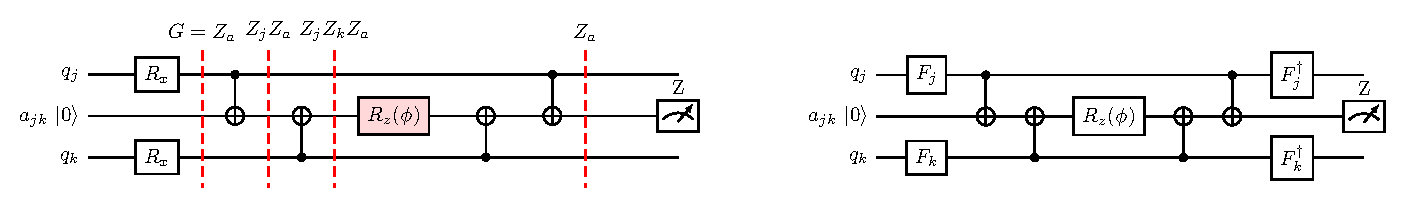
\includegraphics[width=\textwidth]{figs/fig_hw_gadget.pdf}
\caption{Left: the anchor paper's ancilla-mediated bond gadget on heavy-hex. The ancilla $a_{jk}$ sits between the data qubits, computes the $Z_jZ_k$ parity, carries the $R_z(\phi)$ (red), is uncomputed and measured once at the end; the dashed slices give the back-propagated image of the terminal $Z_a$. No extra gate is spent on detection; the flavor is fixed and $Z$-type faults are undetected. Right: the same gadget with single-qubit frame gates $F_j,F_k$ at its boundary. Since the gates sit outside the CX pair, they do not change which physical faults the check sees; the randomization that does is the choice among native \emph{compilations} of the gadget (text).}
\label{fig:hw-gadget}
\end{figure}

\paragraph{A ring with periphery ancillas.} Take $n$ data qubits on a ring with nearest-neighbour CX and one ancilla $a_i$ attached to each $q_i$, with controlled-Paulis only between $a_i$ and $q_i$. On a single wire the only valid check windows are $Z_i$ opened before and closed after the ZZ layer (image $Z_i$, becoming $Z_{i-1}Z_i$ inside the gadget in which $i$ is the CX target) and $X_i$ around the $R_x$ layer: the flavor twirl of the main text is not available. Two cheap randomizations restore a nearly fair coin. (i)~\emph{Enable twirl}: run check $i$ in a given step with probability $b$, independently. (ii)~\emph{Compilation twirl}: the bond gadget has several native two-CX compilations, $CX\,R_z^{(k)}\,CX$ (rotation on the target, the target's check spreads to $Z_jZ_k$ between the CXs), $(H\otimes H)\,CX\,R_x^{(j)}\,CX\,(H\otimes H)$ (rotation on the control, the control's check spreads to $X_jX_k$), and $Y$-type variants; choosing the compilation per gadget per shot changes the Pauli type of the check images \emph{at the CZ noise locations} while the logical gate is unchanged, with the single-qubit conjugations merged into the neighbouring $R_x$ layer (Fig.~\ref{fig:hw-design}). Physical depolarizing faults are type-uniform, so a type-uniform image is anticommuted by any given fault with probability $\tfrac23$, and the former rotation-axis faults are flagged like any other: the invisible sector disappears without repair gates.

\begin{figure}[h]
\centering
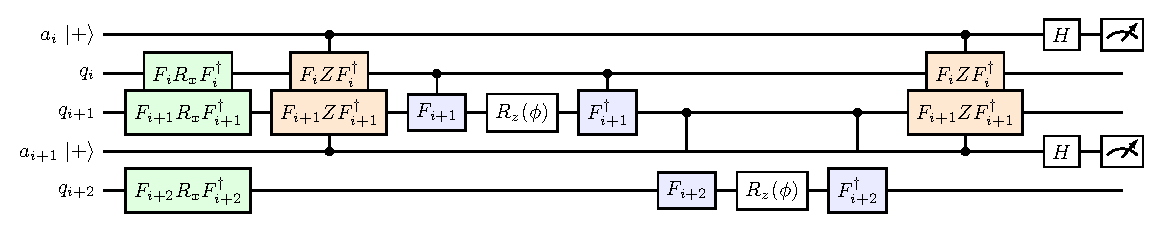
\includegraphics[width=0.95\textwidth]{figs/fig_hw_design.pdf}
\caption{Proposed ring design, one ZZ sub-layer shown. Each data qubit carries a periphery ancilla; check $i$ (enabled with probability $b$) applies a controlled-$F_iZF_i^\dagger$ to its own qubit before and after the ZZ layer, where $F_i$ labels the image type $\{Z,X,Y\}$ realised by the chosen compilation of the gadgets touching $q_i$ (blue single-qubit gates, merged with the $R_x$ layer in green). All two-qubit gates are between adjacent qubits.}
\label{fig:hw-design}
\end{figure}

\begin{table}[h]
\centering\small
\caption{Flag probability of payload faults in a bond gadget for the ring design (\texttt{demo/hw\_coins.py}), image types uniform, compilations equiprobable, enable probability $b$.}
\label{tab:hw-coins}
\begin{tabular}{llcc}
\toprule
location & faults & $b=\tfrac12$ & $b=\tfrac34$ \\
\midrule
after CX2 (and outside the gadgets) & all 15 & $\tfrac13$ / $\tfrac49$ & $\tfrac12$ for all 15 \\
after CX1 (between the CXs) & 6 single-site & $\tfrac13$ & $0.375$ \\
after CX1 & 9 two-site & $\tfrac49$ & $0.583$ \\
data fault right after its own controlled-Pauli & 3 & $\tfrac23$ & $\tfrac23$ \\
ancilla $Z$ or $Y$ in the window & & 1 & 1 \\
ancilla $X$ in the window (branch flip, undetected $P_L$ on data) & & 0 & 0 \\
\bottomrule
\end{tabular}
\end{table}

Table~\ref{tab:hw-coins} gives the coins. With $b=\tfrac34$ half of the payload fault locations carry an exactly fair coin and the other half has mean coin exactly $\tfrac12$ with a spread of $\pm0.1$ between single- and two-site faults. The obstruction to a perfectly uniform coin is structural: between the CXs the only valid image on the idle qubit is $Z$-type, so every check covering that location anticommutes with a given fault in the same way and the two checks' coins are correlated through the shared image rather than independent; no single-wire design removes this, a two-wire ancilla adjacent to both qubits of a bond would. For depolarizing noise the first-order bias of the single-species estimator vanishes because the mean coin is $\tfrac12$ at every location; what remains is the species covariance between coin and the observable's response to single- versus two-site faults, expected at the $10^{-2}$ level at $\Lambda\sim1$ and removable by a two-class stratification, for which the $n$ independent flags per step supply enough acceptance rules. The cost per step for $n=5$, $b=\tfrac34$, is $g=2bn=7.5$ controlled-Paulis, each between an ancilla and its own data qubit, the same count as the all-to-all constrained family but hardware-native and without an invisible payload sector or repair gates; the readout term in (\ref{eq:breakeven}) becomes $bn\,q\,d$, so that at $q=p$ the break-even reads $(\tfrac{14}{15}\cdot17.5+3.75)\,pd\approx20\,pd\lesssim1.2$, the repaired-twirl depth at the constrained-family gate count. Simulating this design on the five-qubit ring (five data and five ancilla qubits, exact density matrix) is the natural next step; the coin table predicts a model-free bias below $10^{-2}$ at the cost of the constrained family.

\paragraph{Fitting the heavy-hex geometry: a 6-ring on one plaquette.} A 5-qubit ring does not exist on heavy-hex: the lattice is bipartite, with degree-3 vertex qubits and degree-2 edge qubits, and its smallest cycle is the 12-qubit plaquette. The natural unit is one plaquette, a ring of \emph{six} data qubits on the vertices with a mediator on every edge, which is the anchor paper's layout, and the third neighbour of every vertex is the edge qubit of the adjacent plaquette, which supplies one peripheral ancilla per data qubit (Fig.~\ref{fig:heavyhex}): 18 qubits, all couplings nearest-neighbour. The payload is then necessarily mediated, 4~CZ per bond and 24~CZ per Trotter step for the 6-ring against 12 for the direct compilation assumed in the main text, and the mediators are free fixed-flavor checks. The mediated gadget has a second native compilation with the mediator as control ($m$ in $|+\rangle$, $CX_{m\to q}$ gates, $R_x^{(m)}$, data in the $H$ frame) in which every image at the CZ noise locations is $X$-type, and a $Y$-type variant; the data frame can even be chosen per qubit, the gadget collecting the parity of the two current-frame operators in 4~CZ. Drawing the compilation per gadget per shot therefore twirls the image type of the mediator check and of the peripheral checks at every noise location, so that no physical fault is invisible, and because each data qubit is the CX control (compilation A) or target (B) of its own parity gate, the peripheral image never spreads onto the neighbouring data qubit: the correlation obstruction of the direct-CX ring does not arise. Table~\ref{tab:hh-coins} gives the resulting flag statistics. With both check types every CZ fault is flagged with probability between $\tfrac12$ and $\tfrac56$ (mean $0.73$) and raises one or two flags; the coin is not uniform, so the single-coin mixture law gives way to a species inversion over classes labelled by coin and flag multiplicity, for which the two independent flag counts per step (6 mediators, up to 6 peripherals) supply two-dimensional threshold rules. The cost is 24 CZ of mediated payload, $2bn=9$ CZ of peripheral checks and $10.5$ readouts per step; the break-even bookkeeping on this geometry, $\tfrac{14}{15}(24+9)pd+10.5\,qd\approx41\,pd\lesssim1.2$, gives $pd\lesssim0.03$, half the direct-CX depth, a cost that the mediated payload imposes on every method alike. The natural simulation is a fault-path Monte Carlo (Pauli faults sampled from the model, flags from the image rule, a 6-qubit statevector for the data), since the 18-qubit density matrix is out of reach.

\begin{figure}[h]
\centering
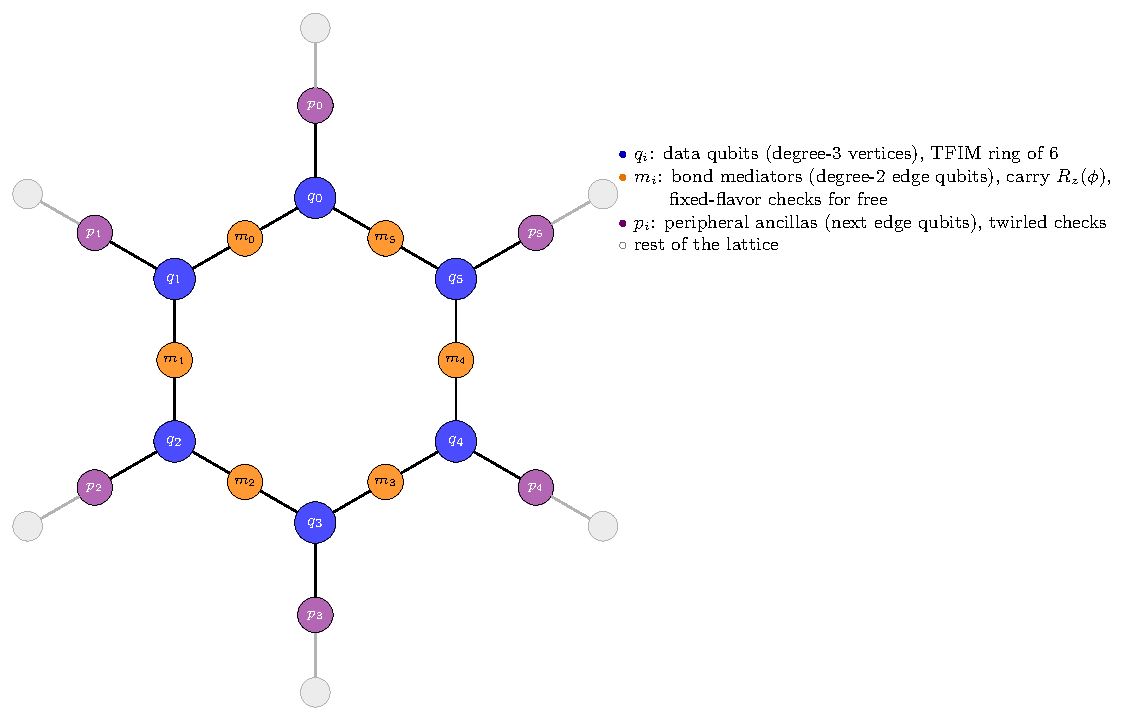
\includegraphics[width=0.85\textwidth]{figs/fig_heavyhex.pdf}
\caption{The 18-qubit heavy-hex patch: six data qubits $q_i$ on the vertices of one plaquette (TFIM ring of 6), six mediators $m_i$ on its edges (bond gadgets and free fixed-flavor checks), six peripheral ancillas $p_i$ on the outgoing edges (twirled single-wire checks). Grey: the rest of the lattice.}
\label{fig:heavyhex}
\end{figure}

\begin{table}[h]
\centering\small
\caption{Probability that a two-qubit depolarizing fault after each CX of the mediated gadget raises at least one flag (\texttt{demo/hw\_coins\_mediated.py}), image types uniform, peripheral enable probability $b$.}
\label{tab:hh-coins}
\begin{tabular}{lccl}
\toprule
checks used & after CX \#1, \#2 & after CX \#3, \#4 & invisible \\
\midrule
mediators only, compilation-twirled & $\tfrac23$ / $\tfrac49$ & $\tfrac23$ / $0$ & data-only faults after the uncompute CXs \\
mediators $+$ peripheral, $b=\tfrac34$ & $\tfrac23$--$0.78$ & $0.5$--$0.83$ & none \\
peripheral only, $b=\tfrac34$ & $\tfrac12$ / $0$ & $\tfrac12$ / $0$ & mediator-only faults \\
\bottomrule
\end{tabular}
\end{table}

\end{document}
